
		\begin{figure}
			\centering
			\subfloat[SHREK]{
				\scalebox{.4}{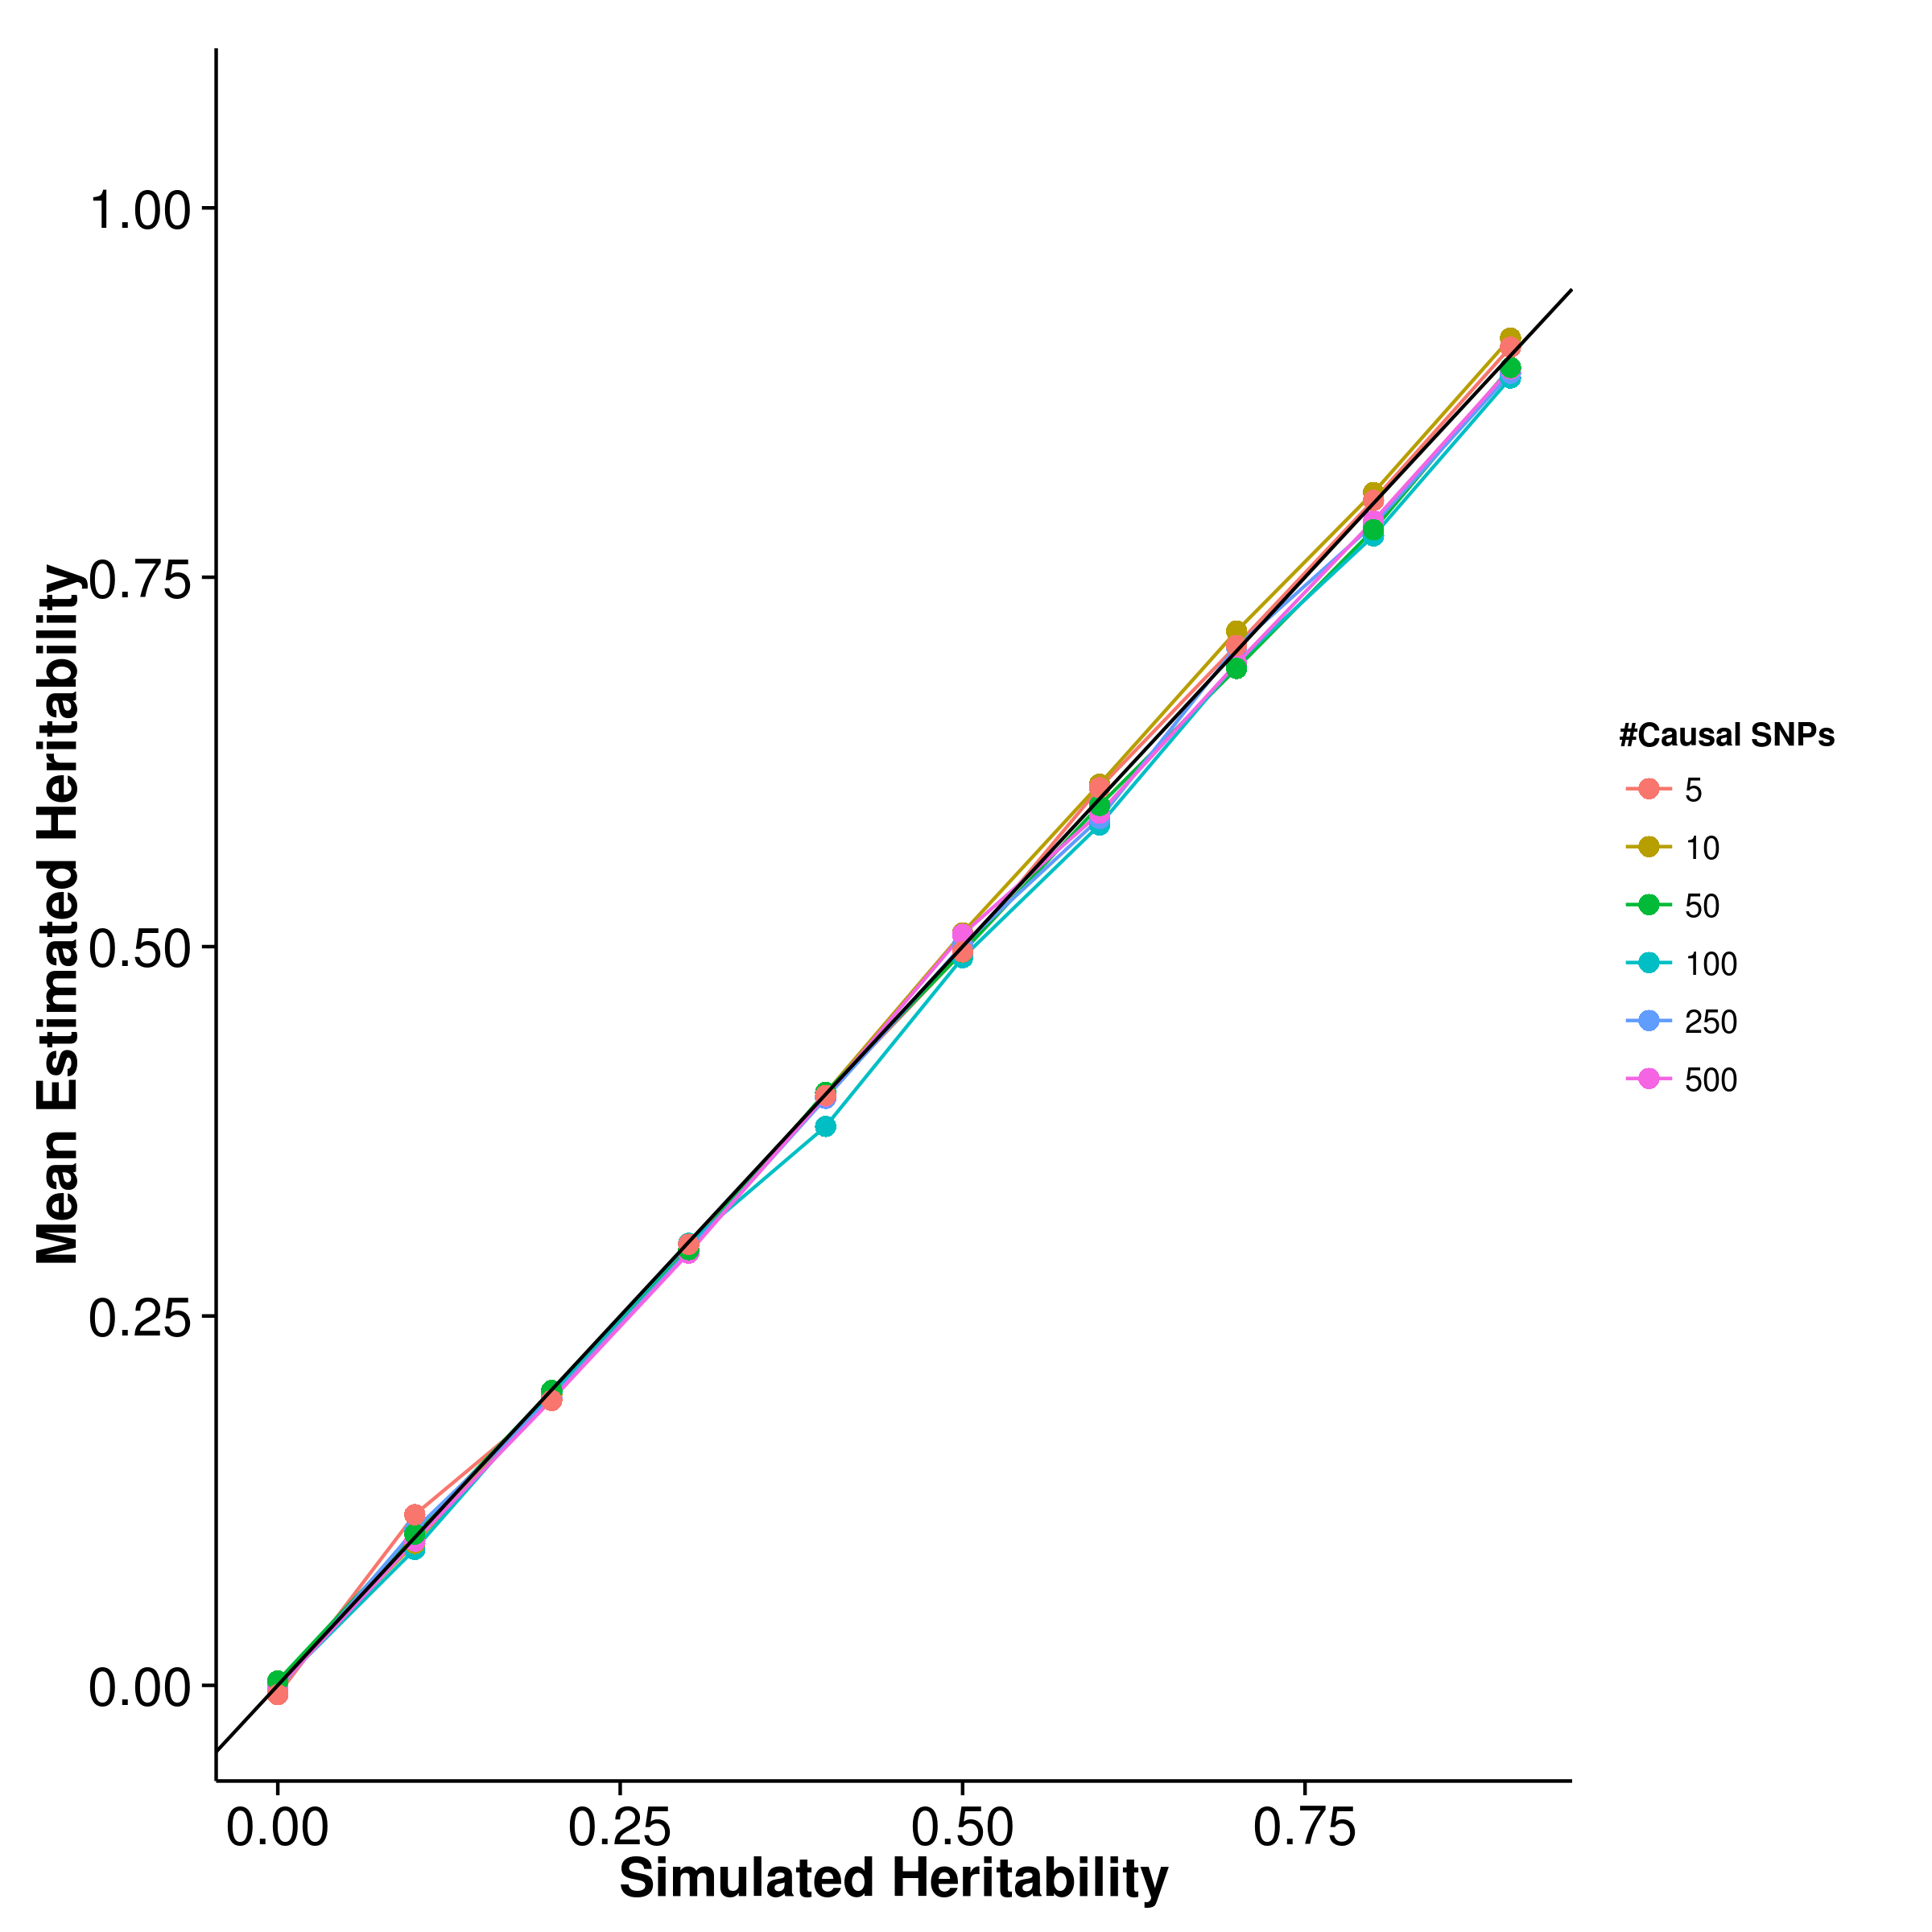
\includegraphics{figure/he_summary/equal/shrek_Qt_Equal_mean.png}}
				\label{fig:shrekQtEqualMean}
			}
			\subfloat[GCTA]{
				\scalebox{.4}{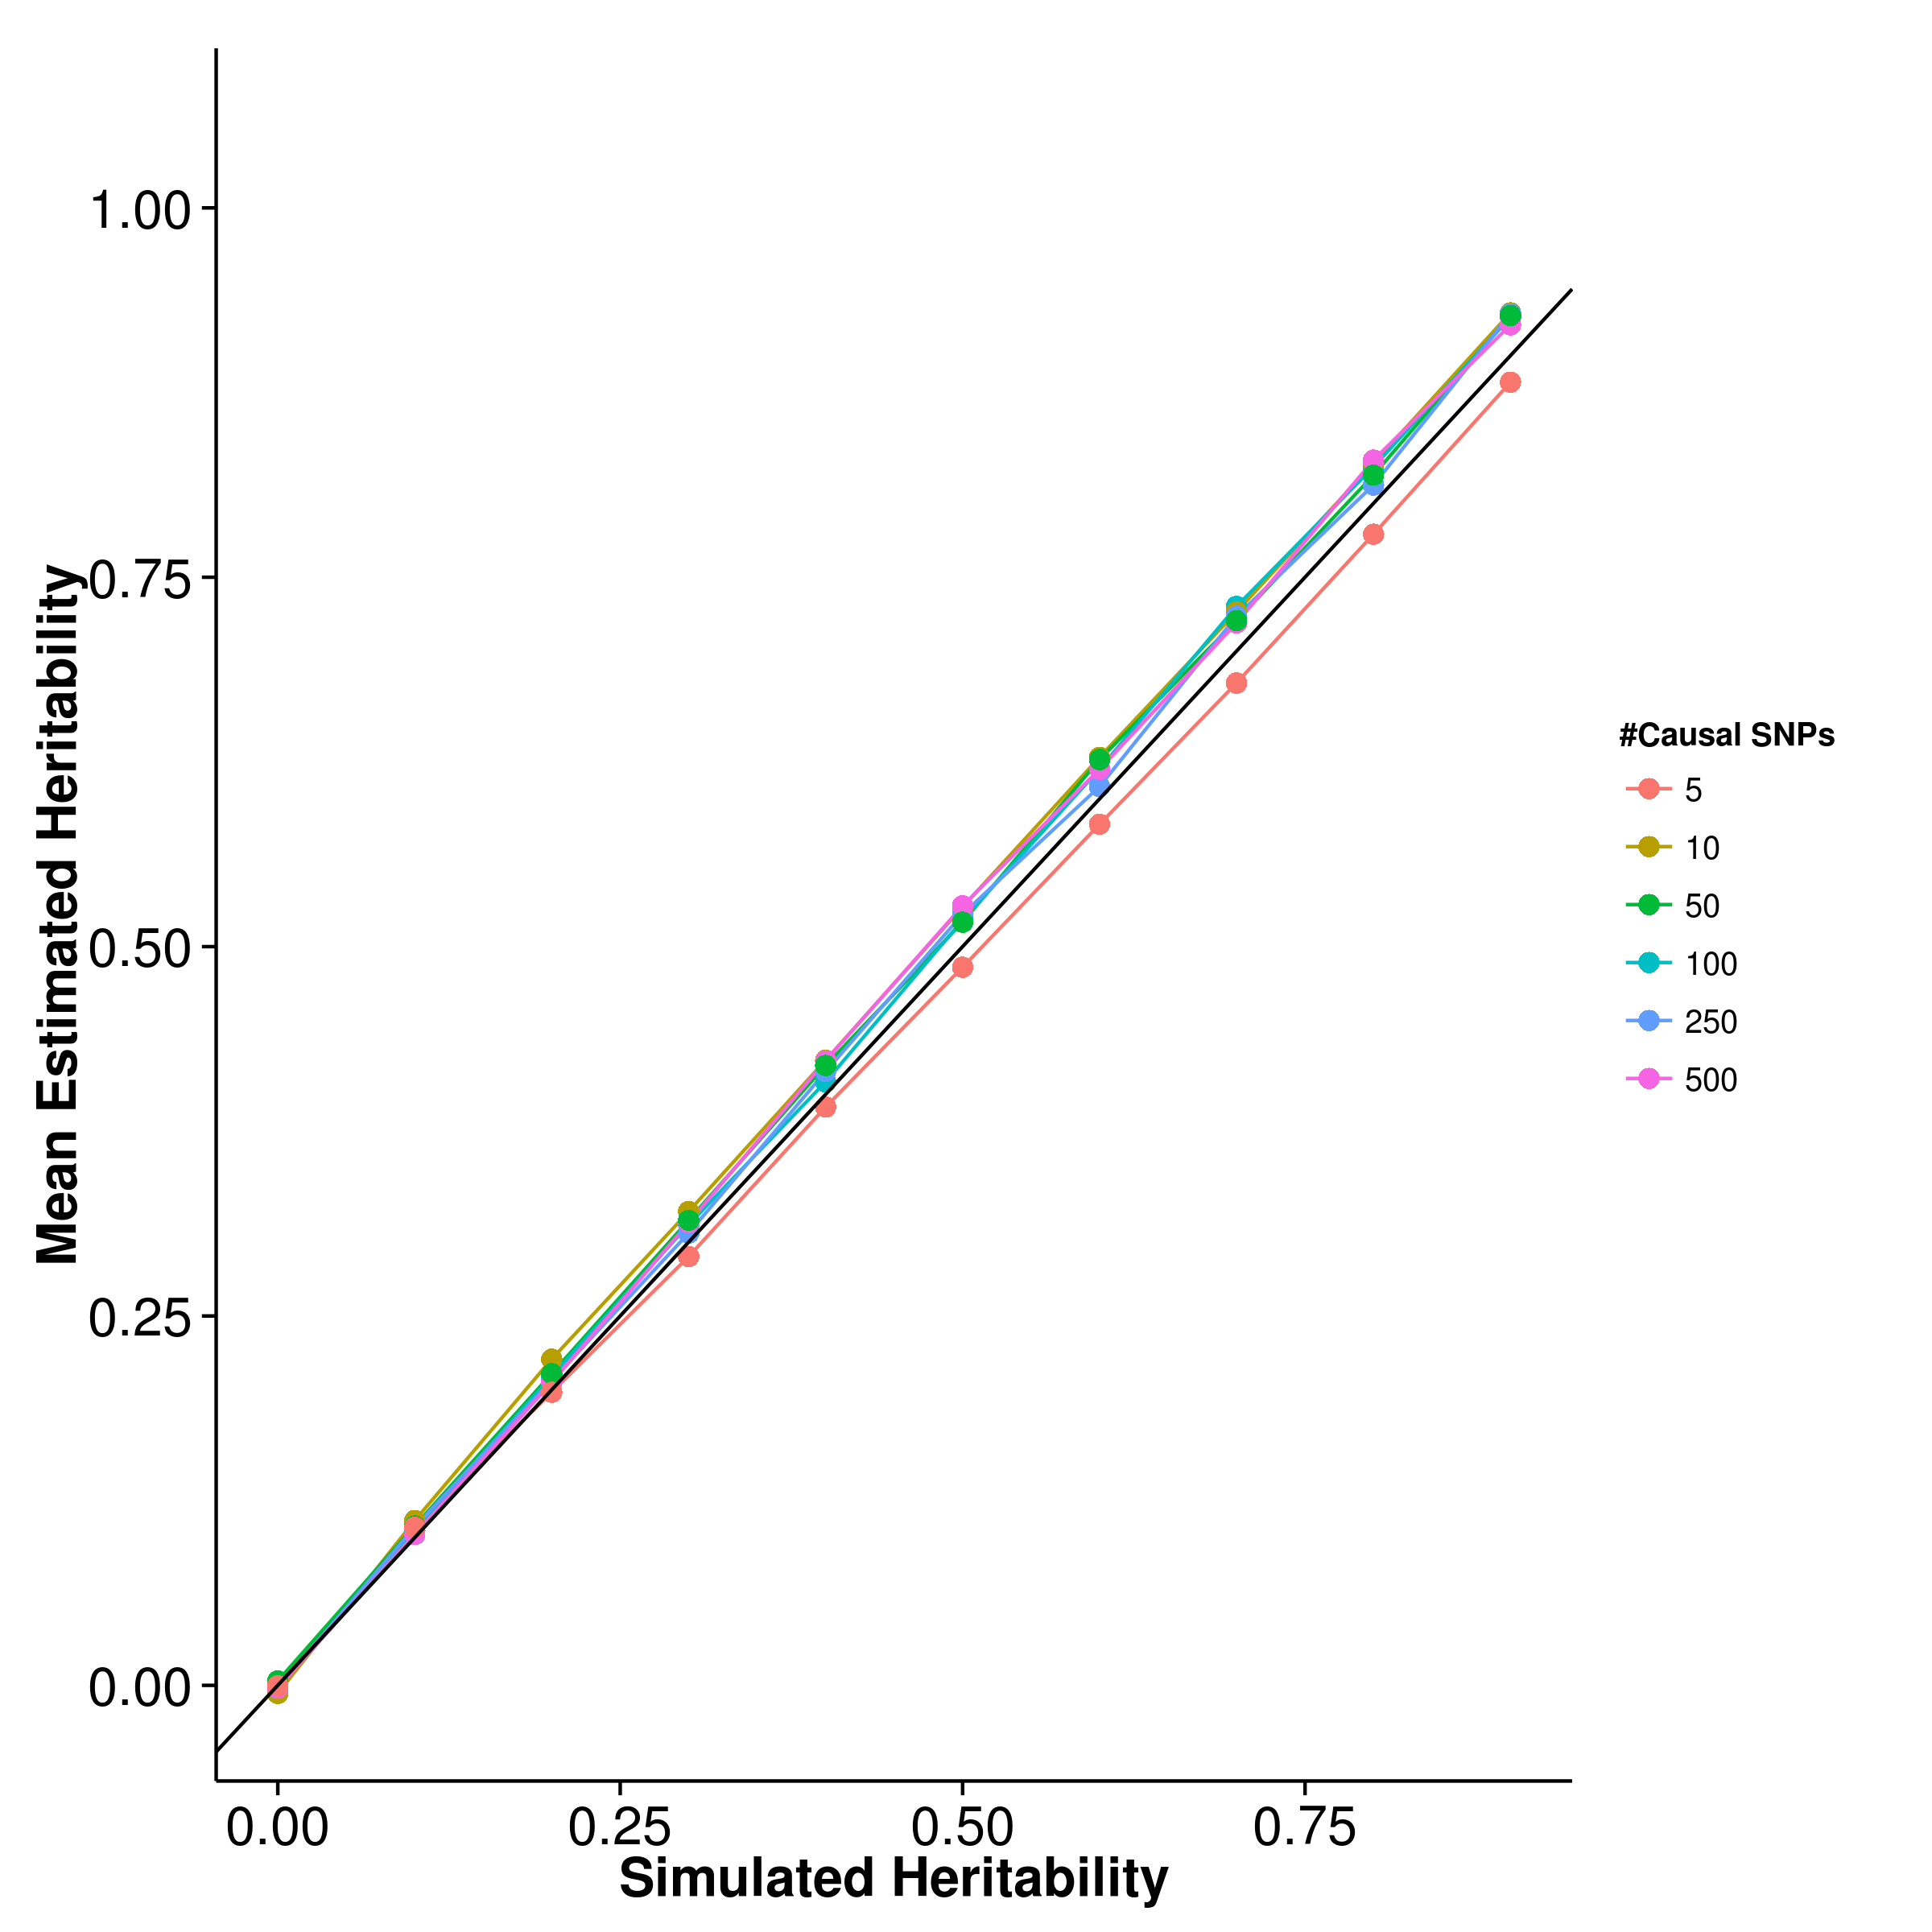
\includegraphics{figure/he_summary/equal/gcta_Qt_Equal_mean.png}}
				\label{fig:gctaQtEqualMean}
			}\\
			\subfloat[LDSC with fix intercept]{
				\scalebox{.4}{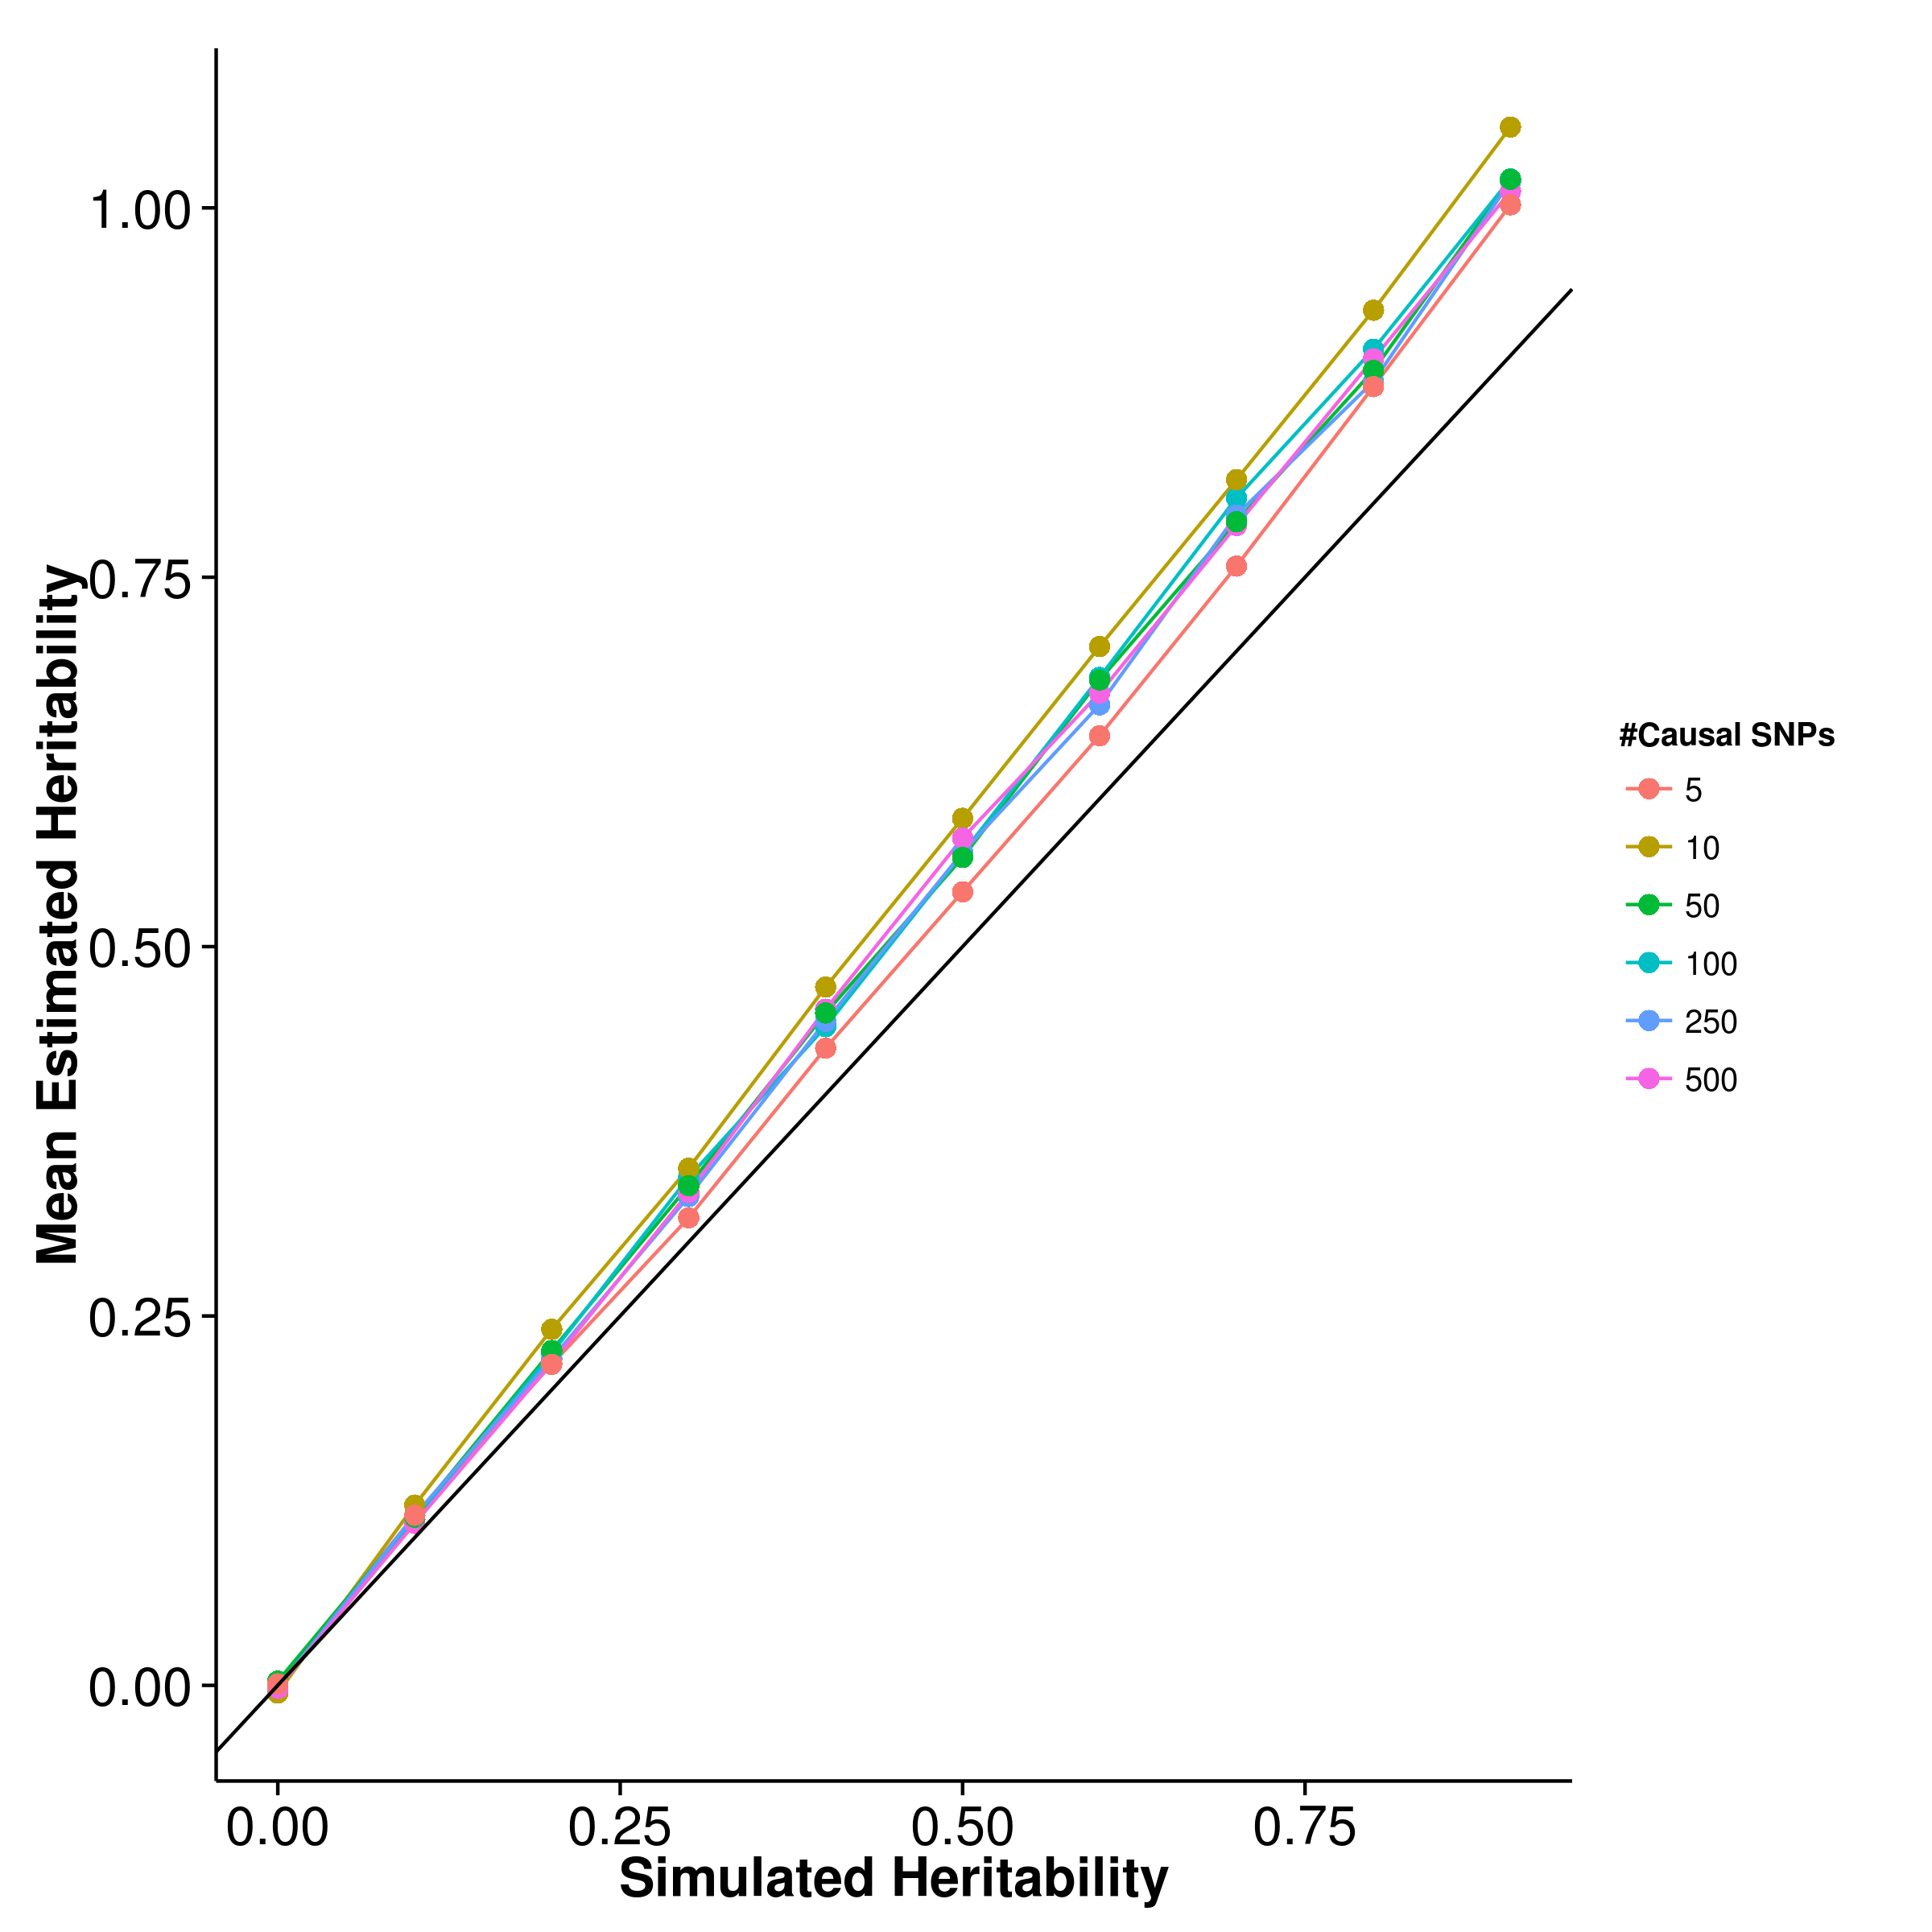
\includegraphics{figure/he_summary/equal/ldsc_Qt_Equal_mean.png}}
				\label{fig:ldscQtEqualMean}
			}
			\subfloat[LDSC with intercept estimation]{
				
				\scalebox{.4}{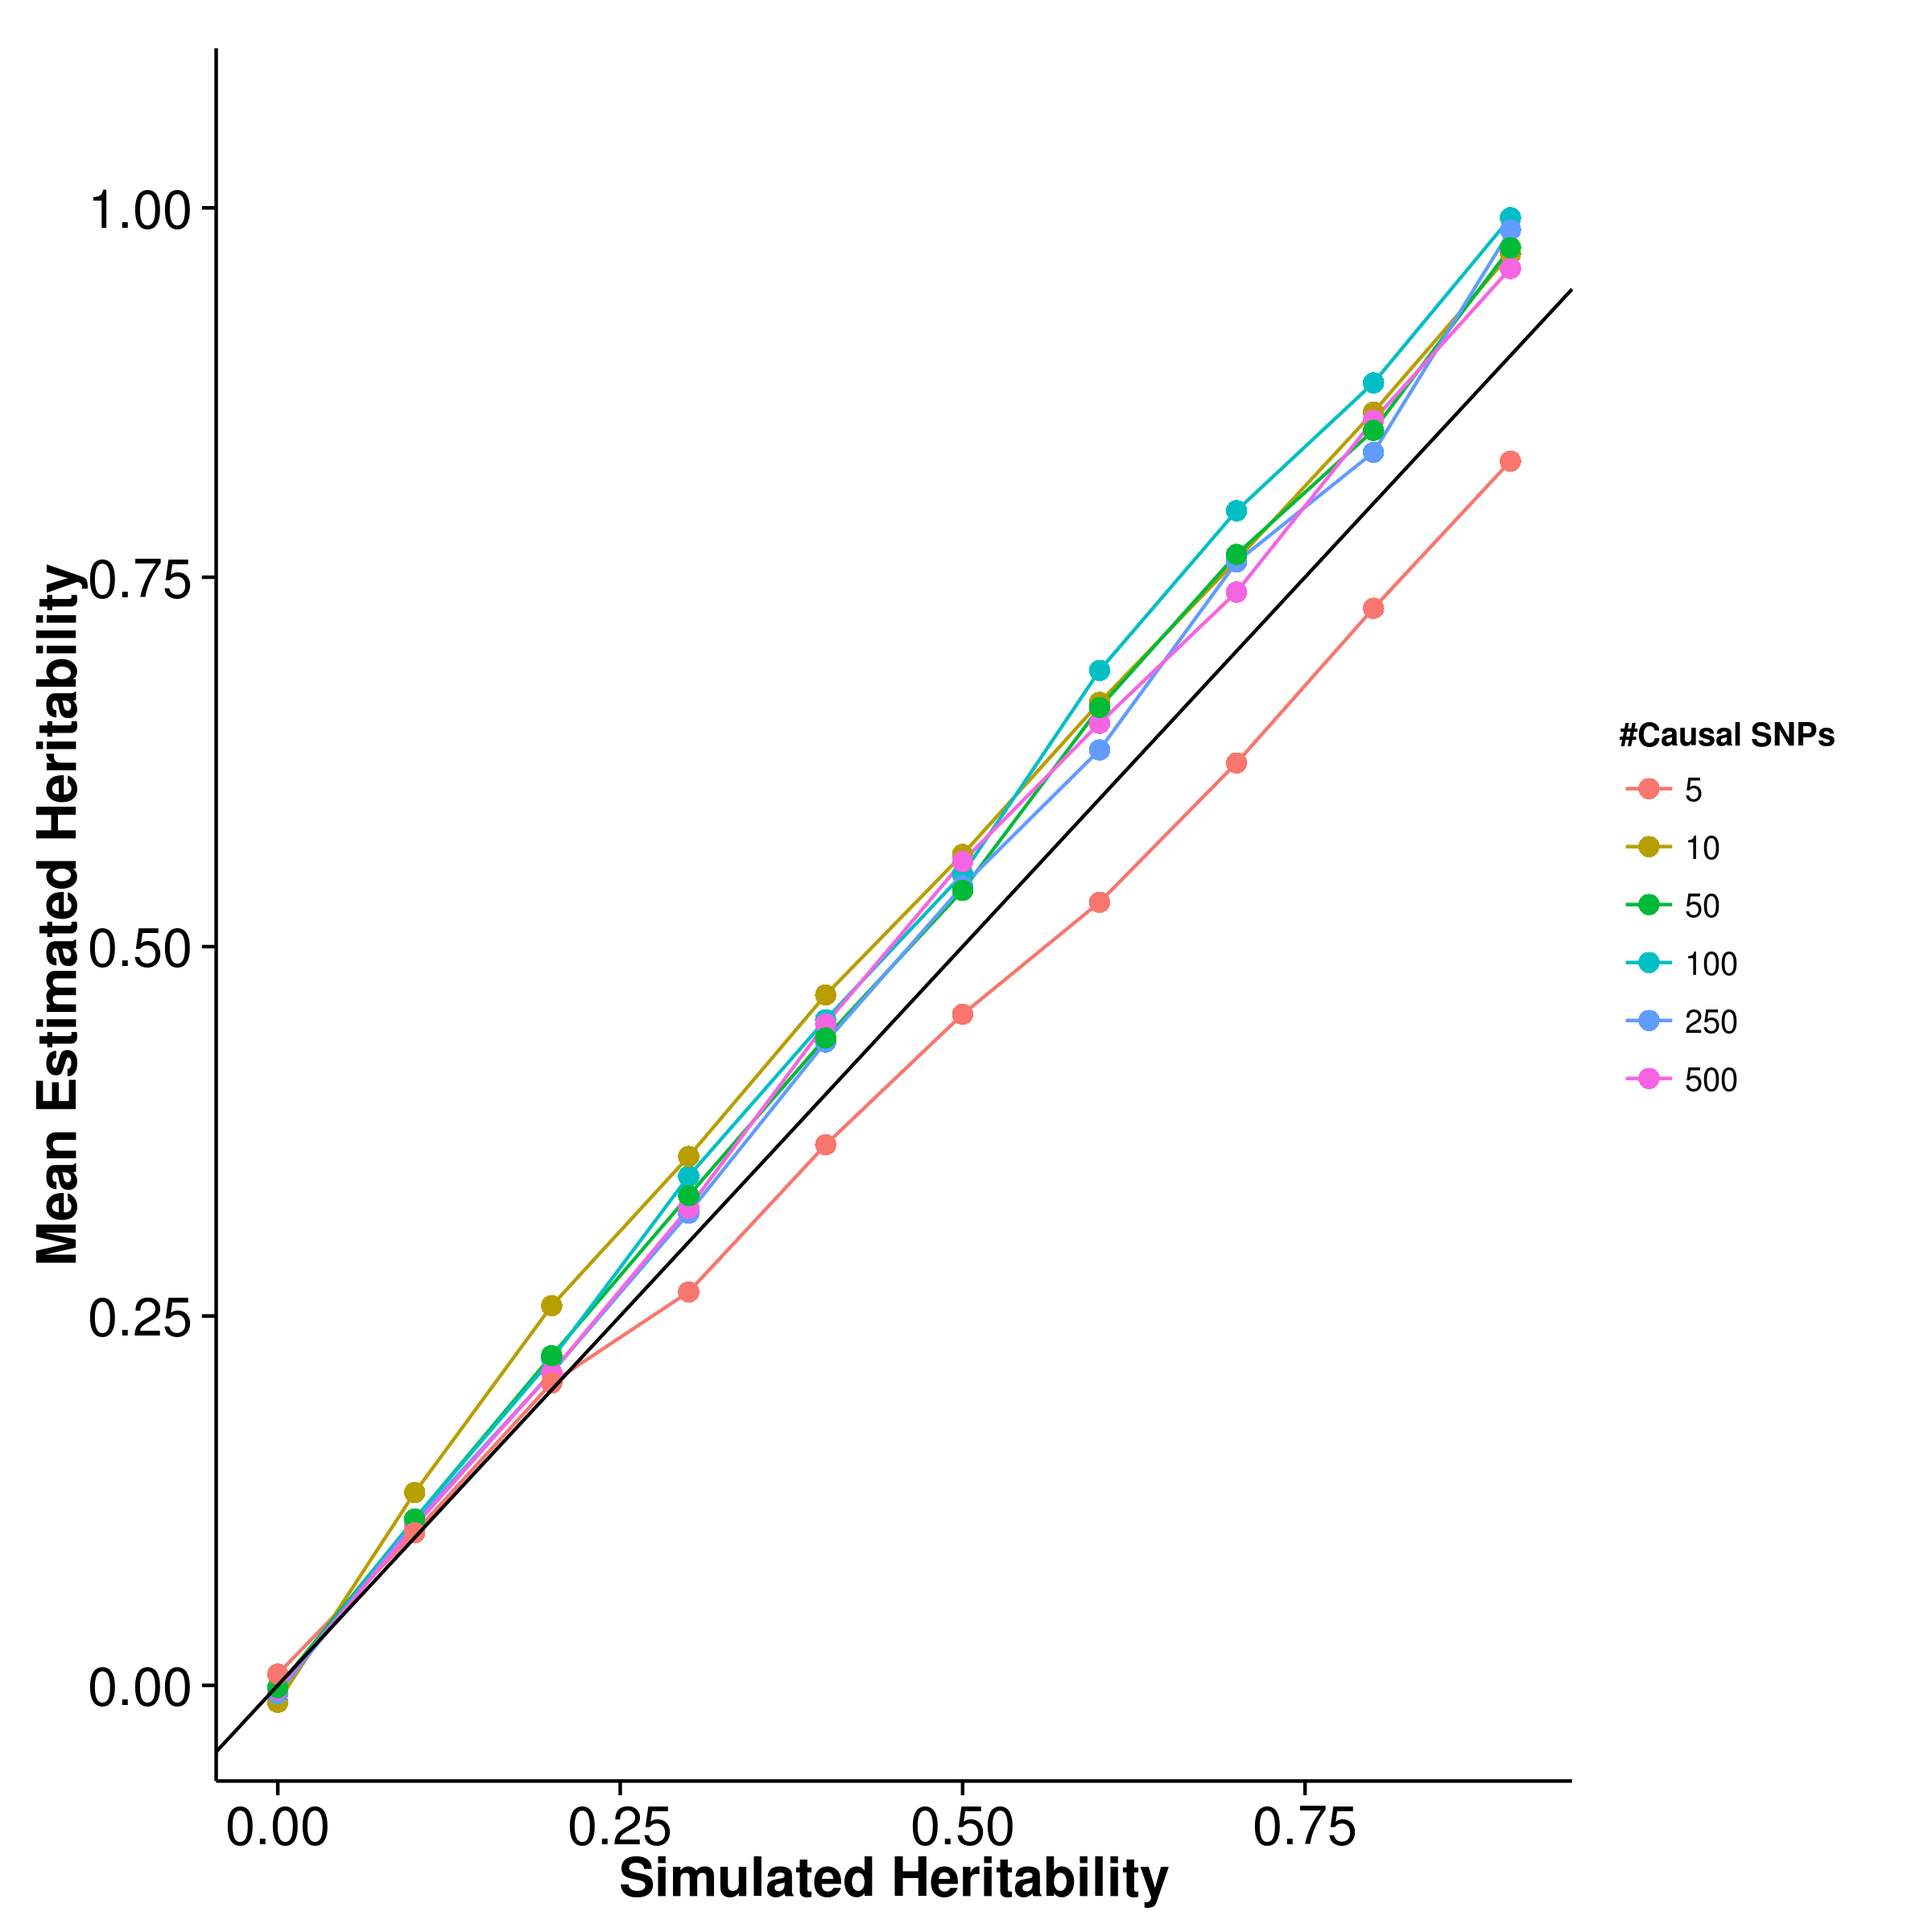
\includegraphics{figure/he_summary/equal/ldscIn_Qt_Equal_mean.png}}
				\label{fig:ldscInQtEqualMean}
			}
			\caption[Quantitative Trait with Equal Effect Size Simulation Result(Mean)]
			{Mean of results from quantitative trait simulation with equal effect size simulation.
				\gls{shrek} was found to be less biased of all the tools whereas there was a slight upward bias for \gls{ldsc} when the intercept was fixed, especially when the number of causal \glspl{SNP} was small.} 
			\label{fig:QtEqualMean}
		\end{figure}
		
		\begin{figure}
			\centering
			\subfloat[SHREK]{
				\scalebox{.4}{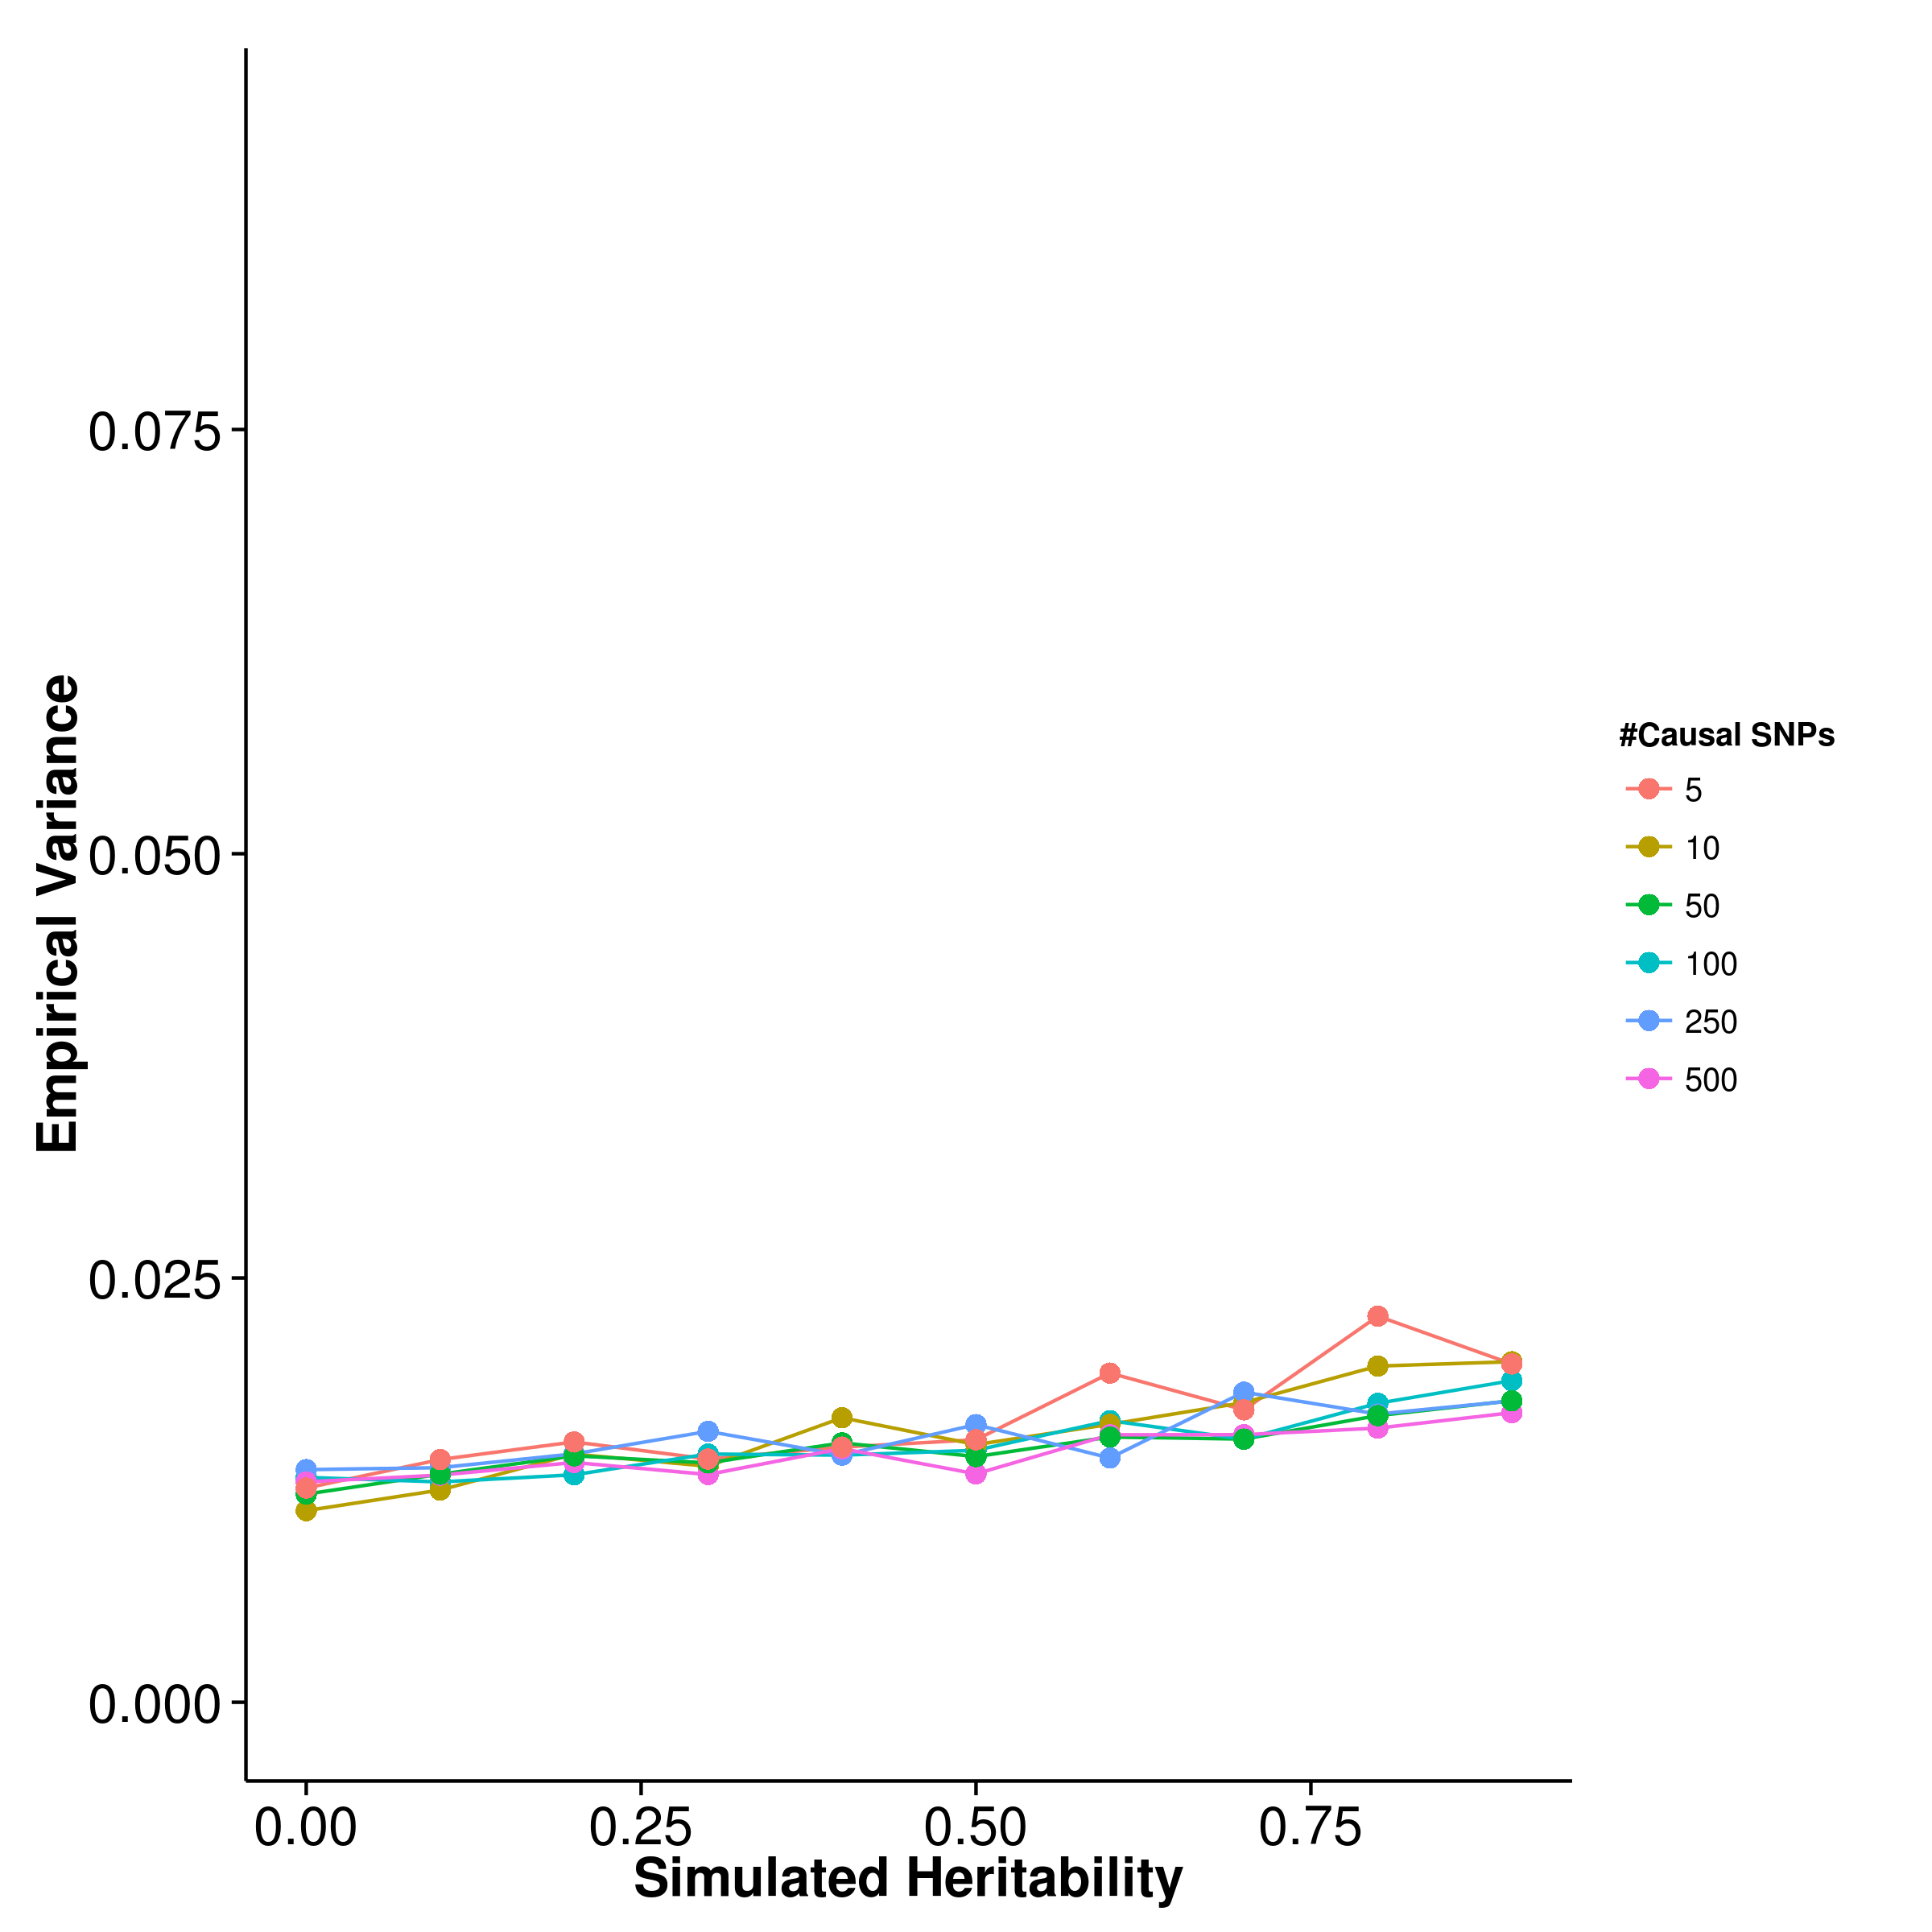
\includegraphics{figure/he_summary/equal/shrek_Qt_Equal_sd.png}}
				\label{fig:shrekQtEqualVar}
			}
			\subfloat[GCTA]{
				\scalebox{.4}{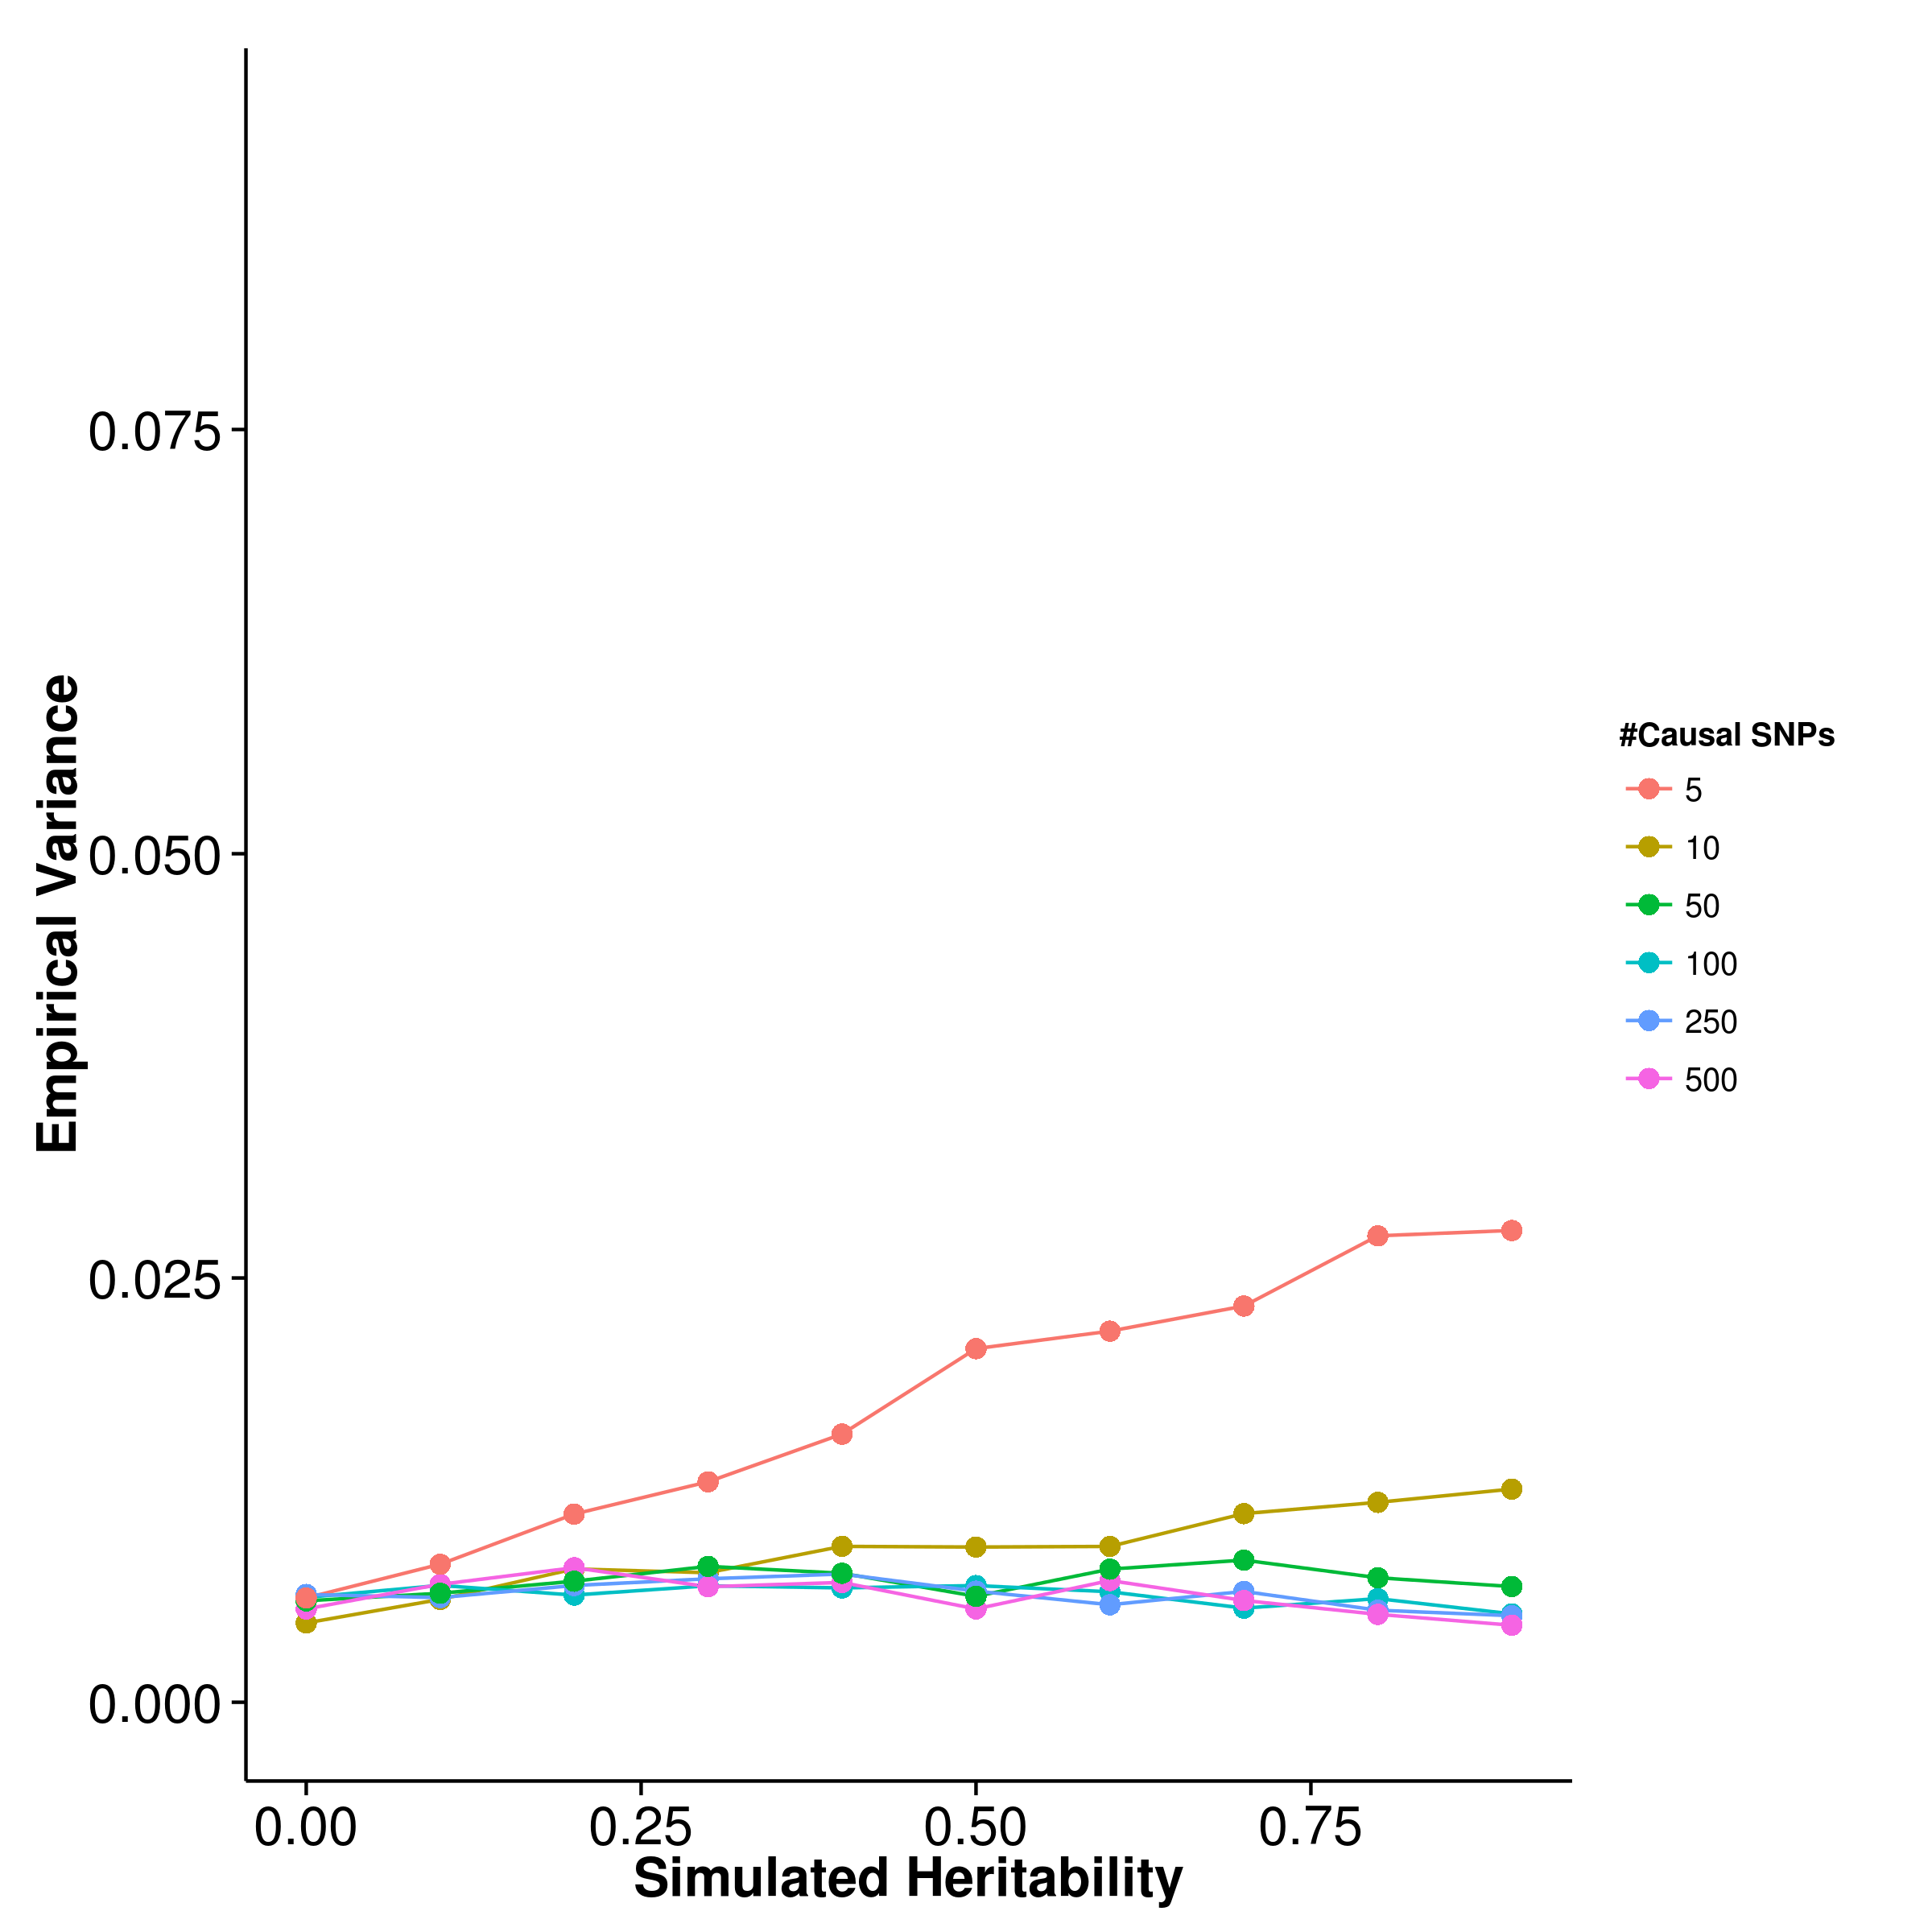
\includegraphics{figure/he_summary/equal/gcta_Qt_Equal_sd.png}}
				\label{fig:gctaQtEqualVar}
			}\\
			\subfloat[LDSC with fix intercept]{
				\scalebox{.4}{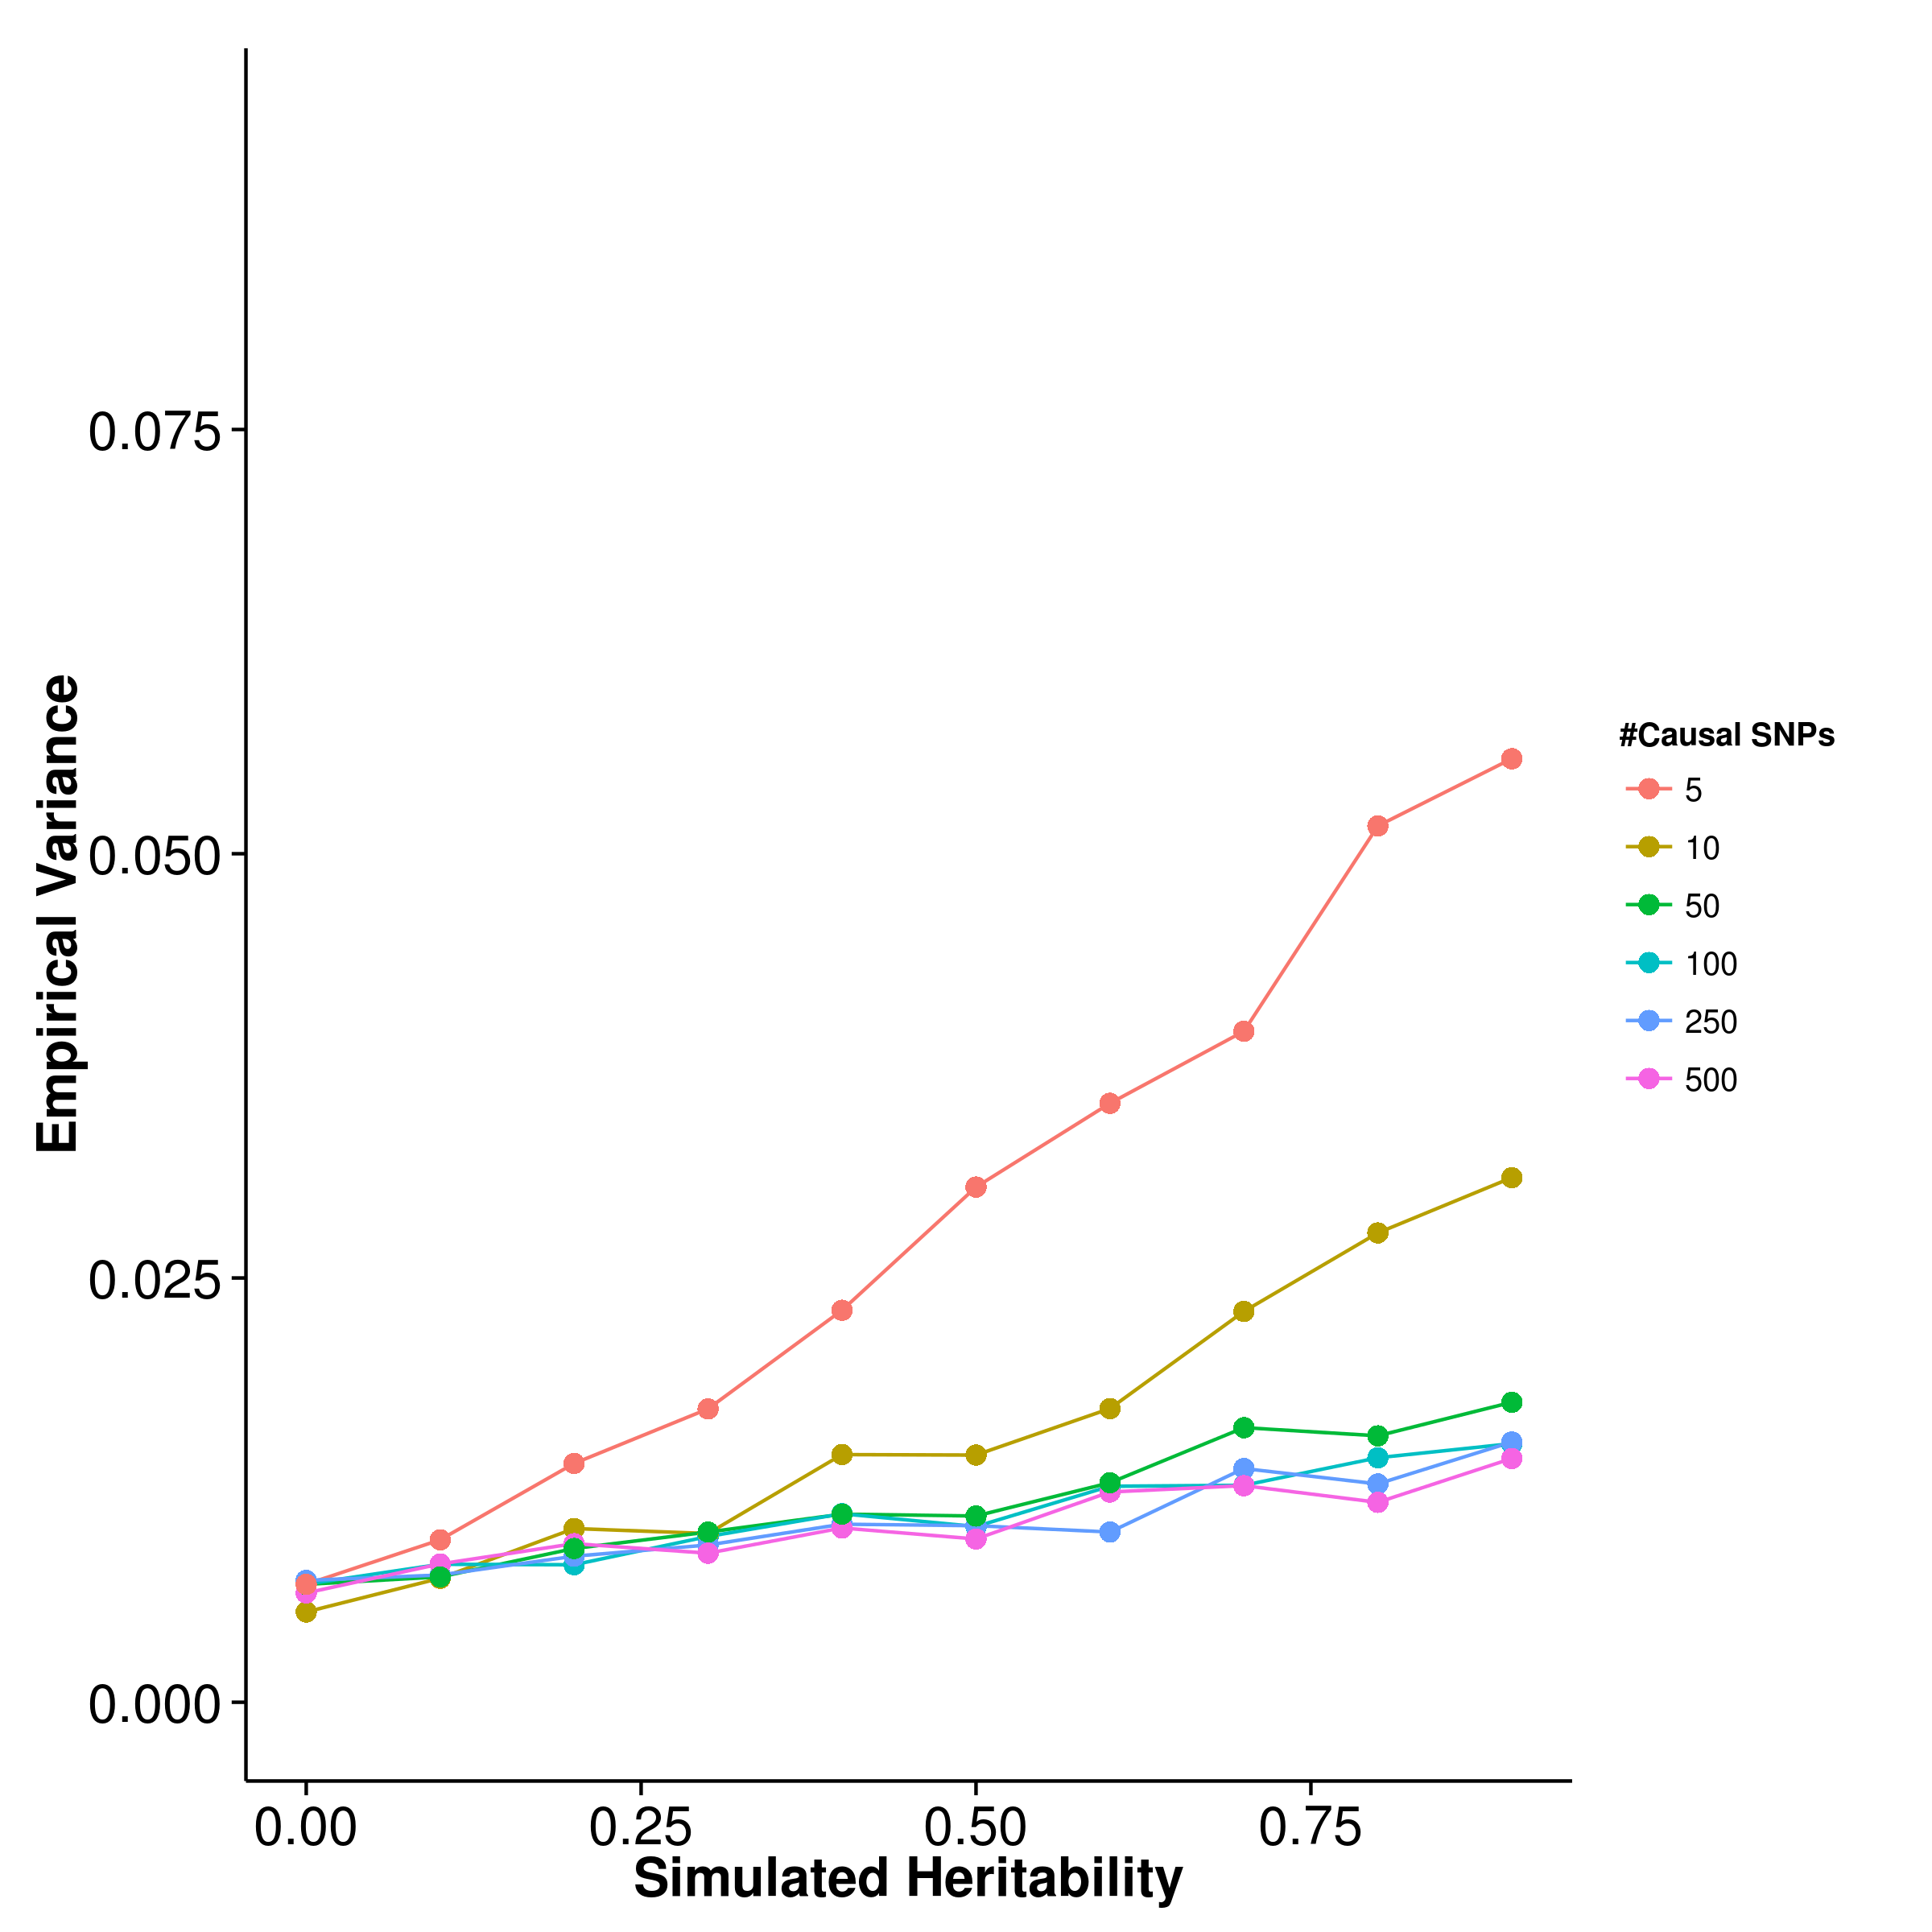
\includegraphics{figure/he_summary/equal/ldsc_Qt_Equal_sd.png}}
				\label{fig:ldscQtEqualVar}
			}
			\subfloat[LDSC with intercept estimation]{
				
				\scalebox{.4}{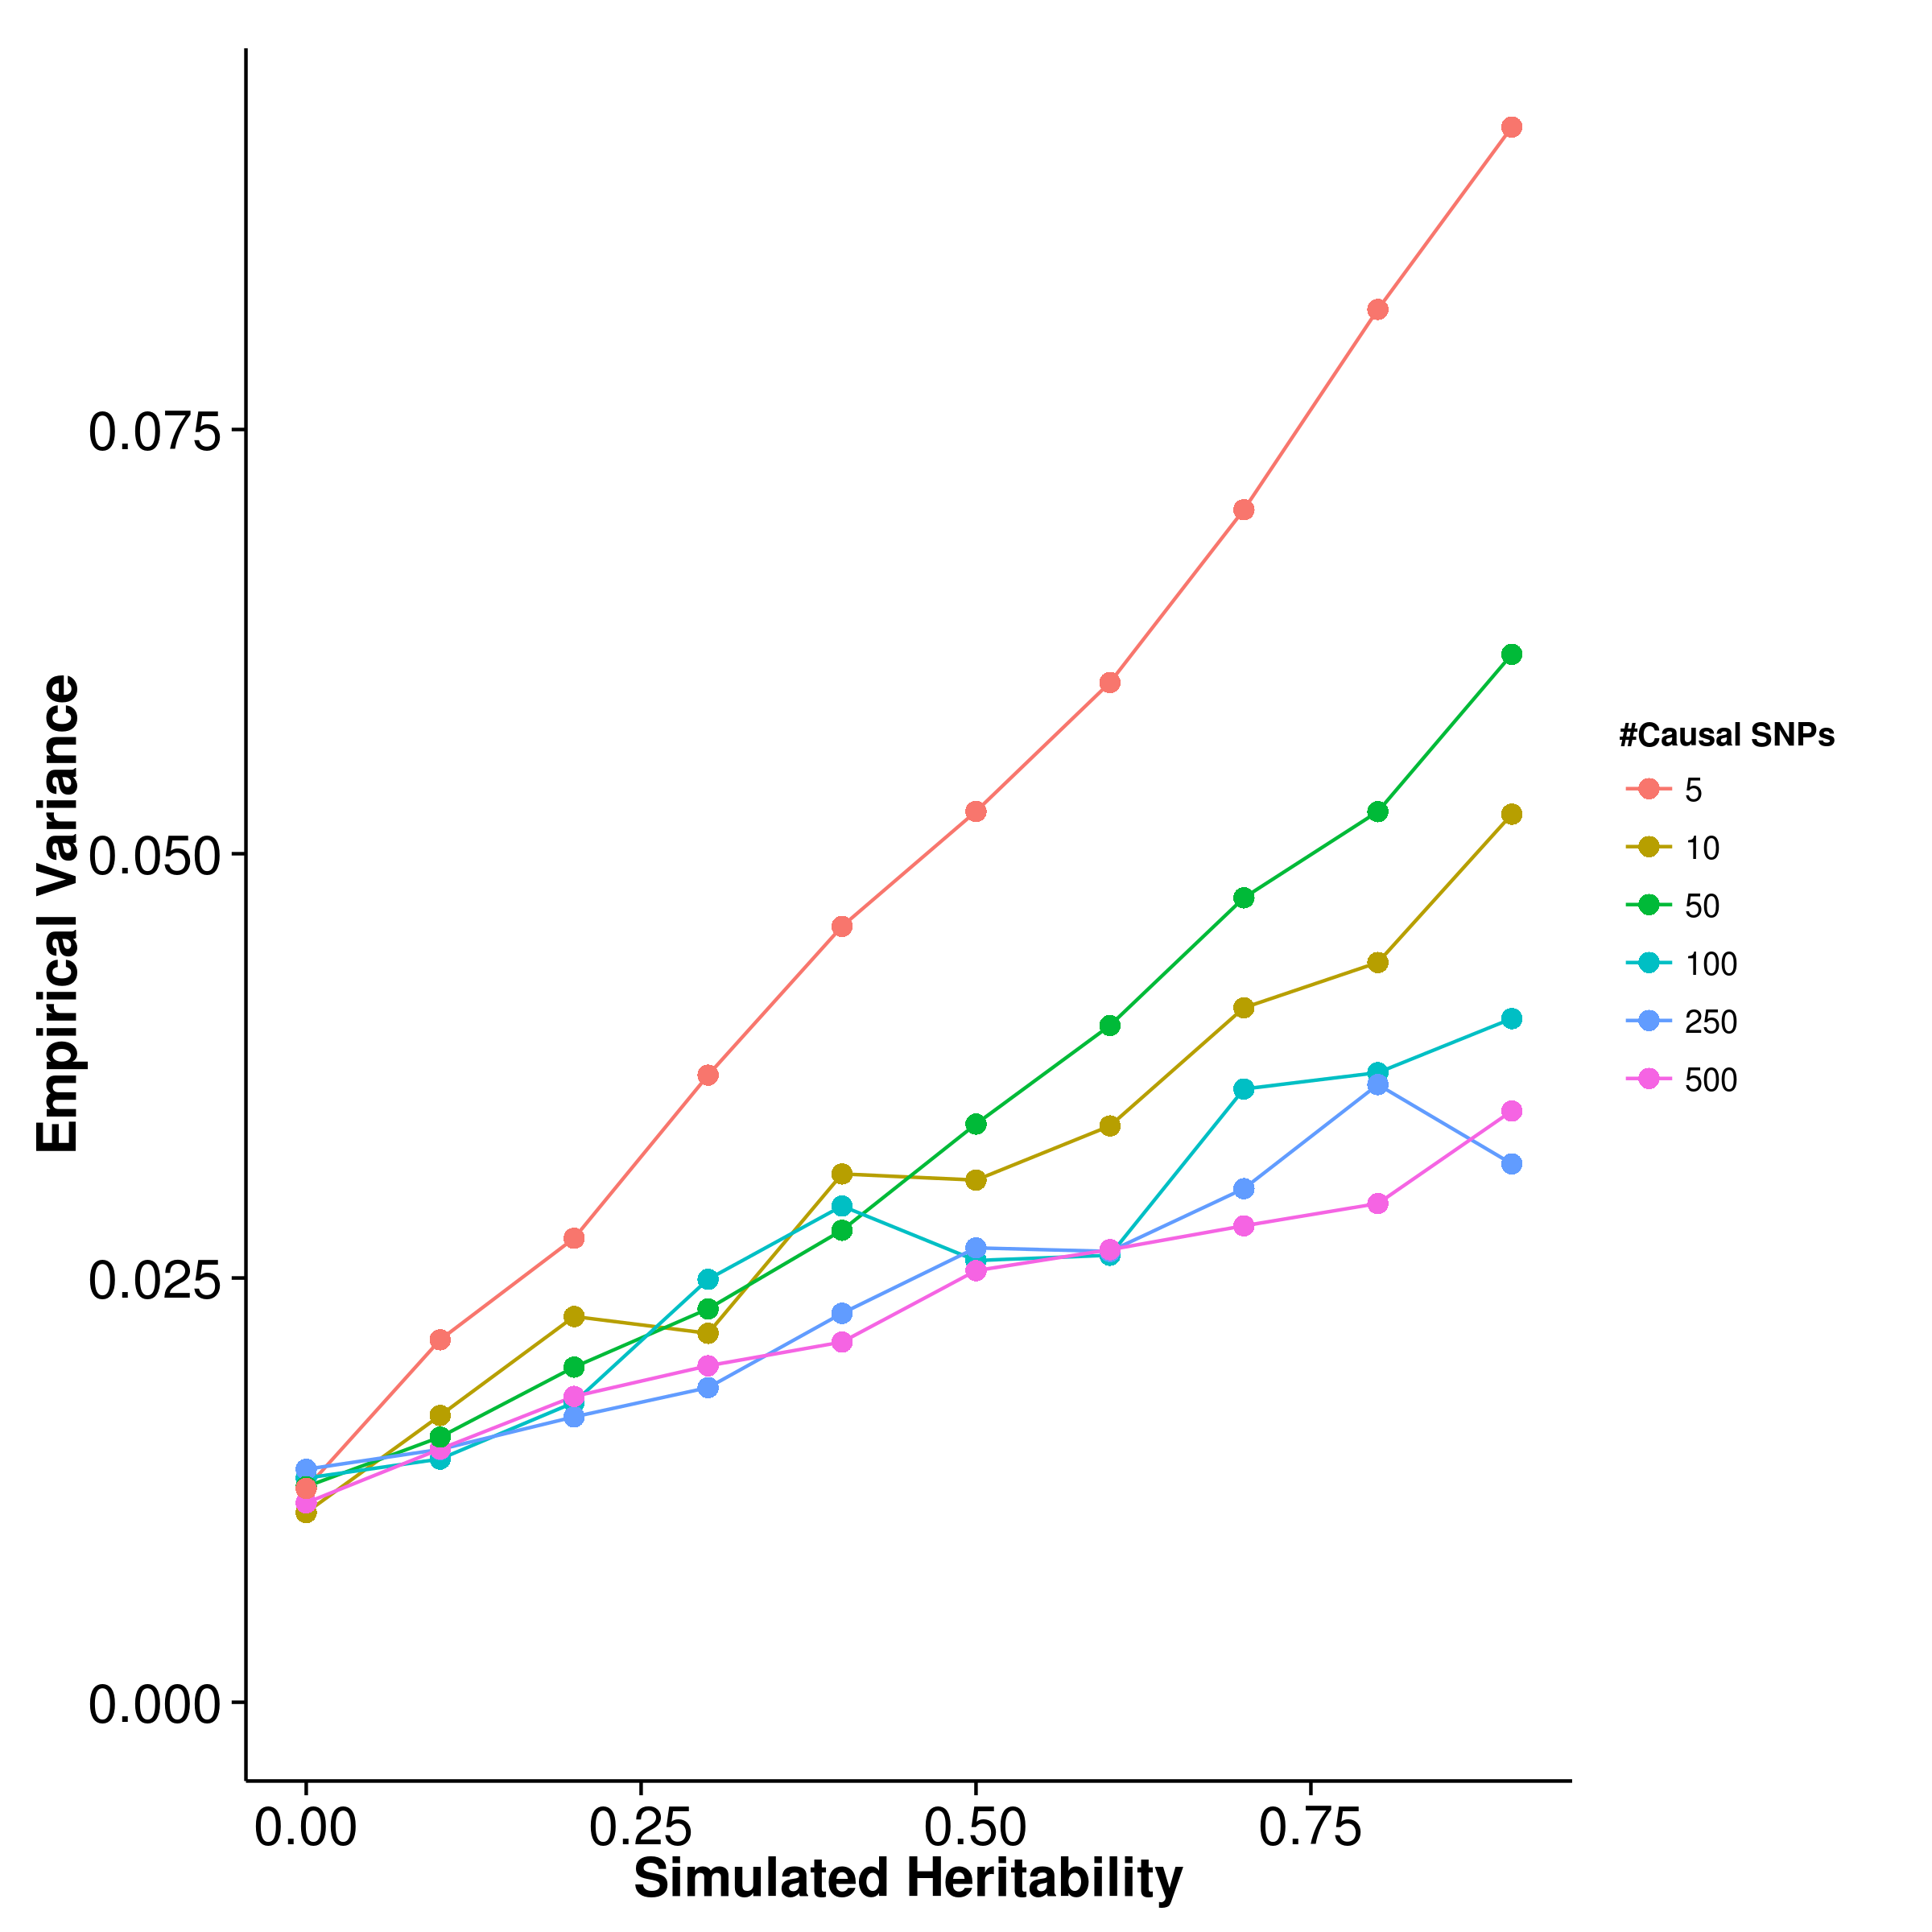
\includegraphics{figure/he_summary/equal/ldscIn_Qt_Equal_sd.png}}
				\label{fig:ldscInQtEqualVar}
			}
			\caption[Quantitative Trait with Equal Effect Size Simulation Result(Variance)]
			{Variance of results from quantitative trait simulation with equal effect size simulation.
				Of all the programmes, \gls{gcta} was found to have the lowest variance, follow by \gls{ldsc} with fixed intercept.
				The variance of \gls{shrek} was slightly higher than that of \gls{ldsc} with fixed intercept and is lower than that of \gls{ldsc} with intercept estimation.
				Unlike \gls{ldsc}, the variance of \gls{shrek} was less sensitive to change in total heritability.} 
			\label{fig:QtEqualVar}
		\end{figure}
		
		\begin{figure}
			\centering
			\subfloat[SHREK]{
				\scalebox{.4}{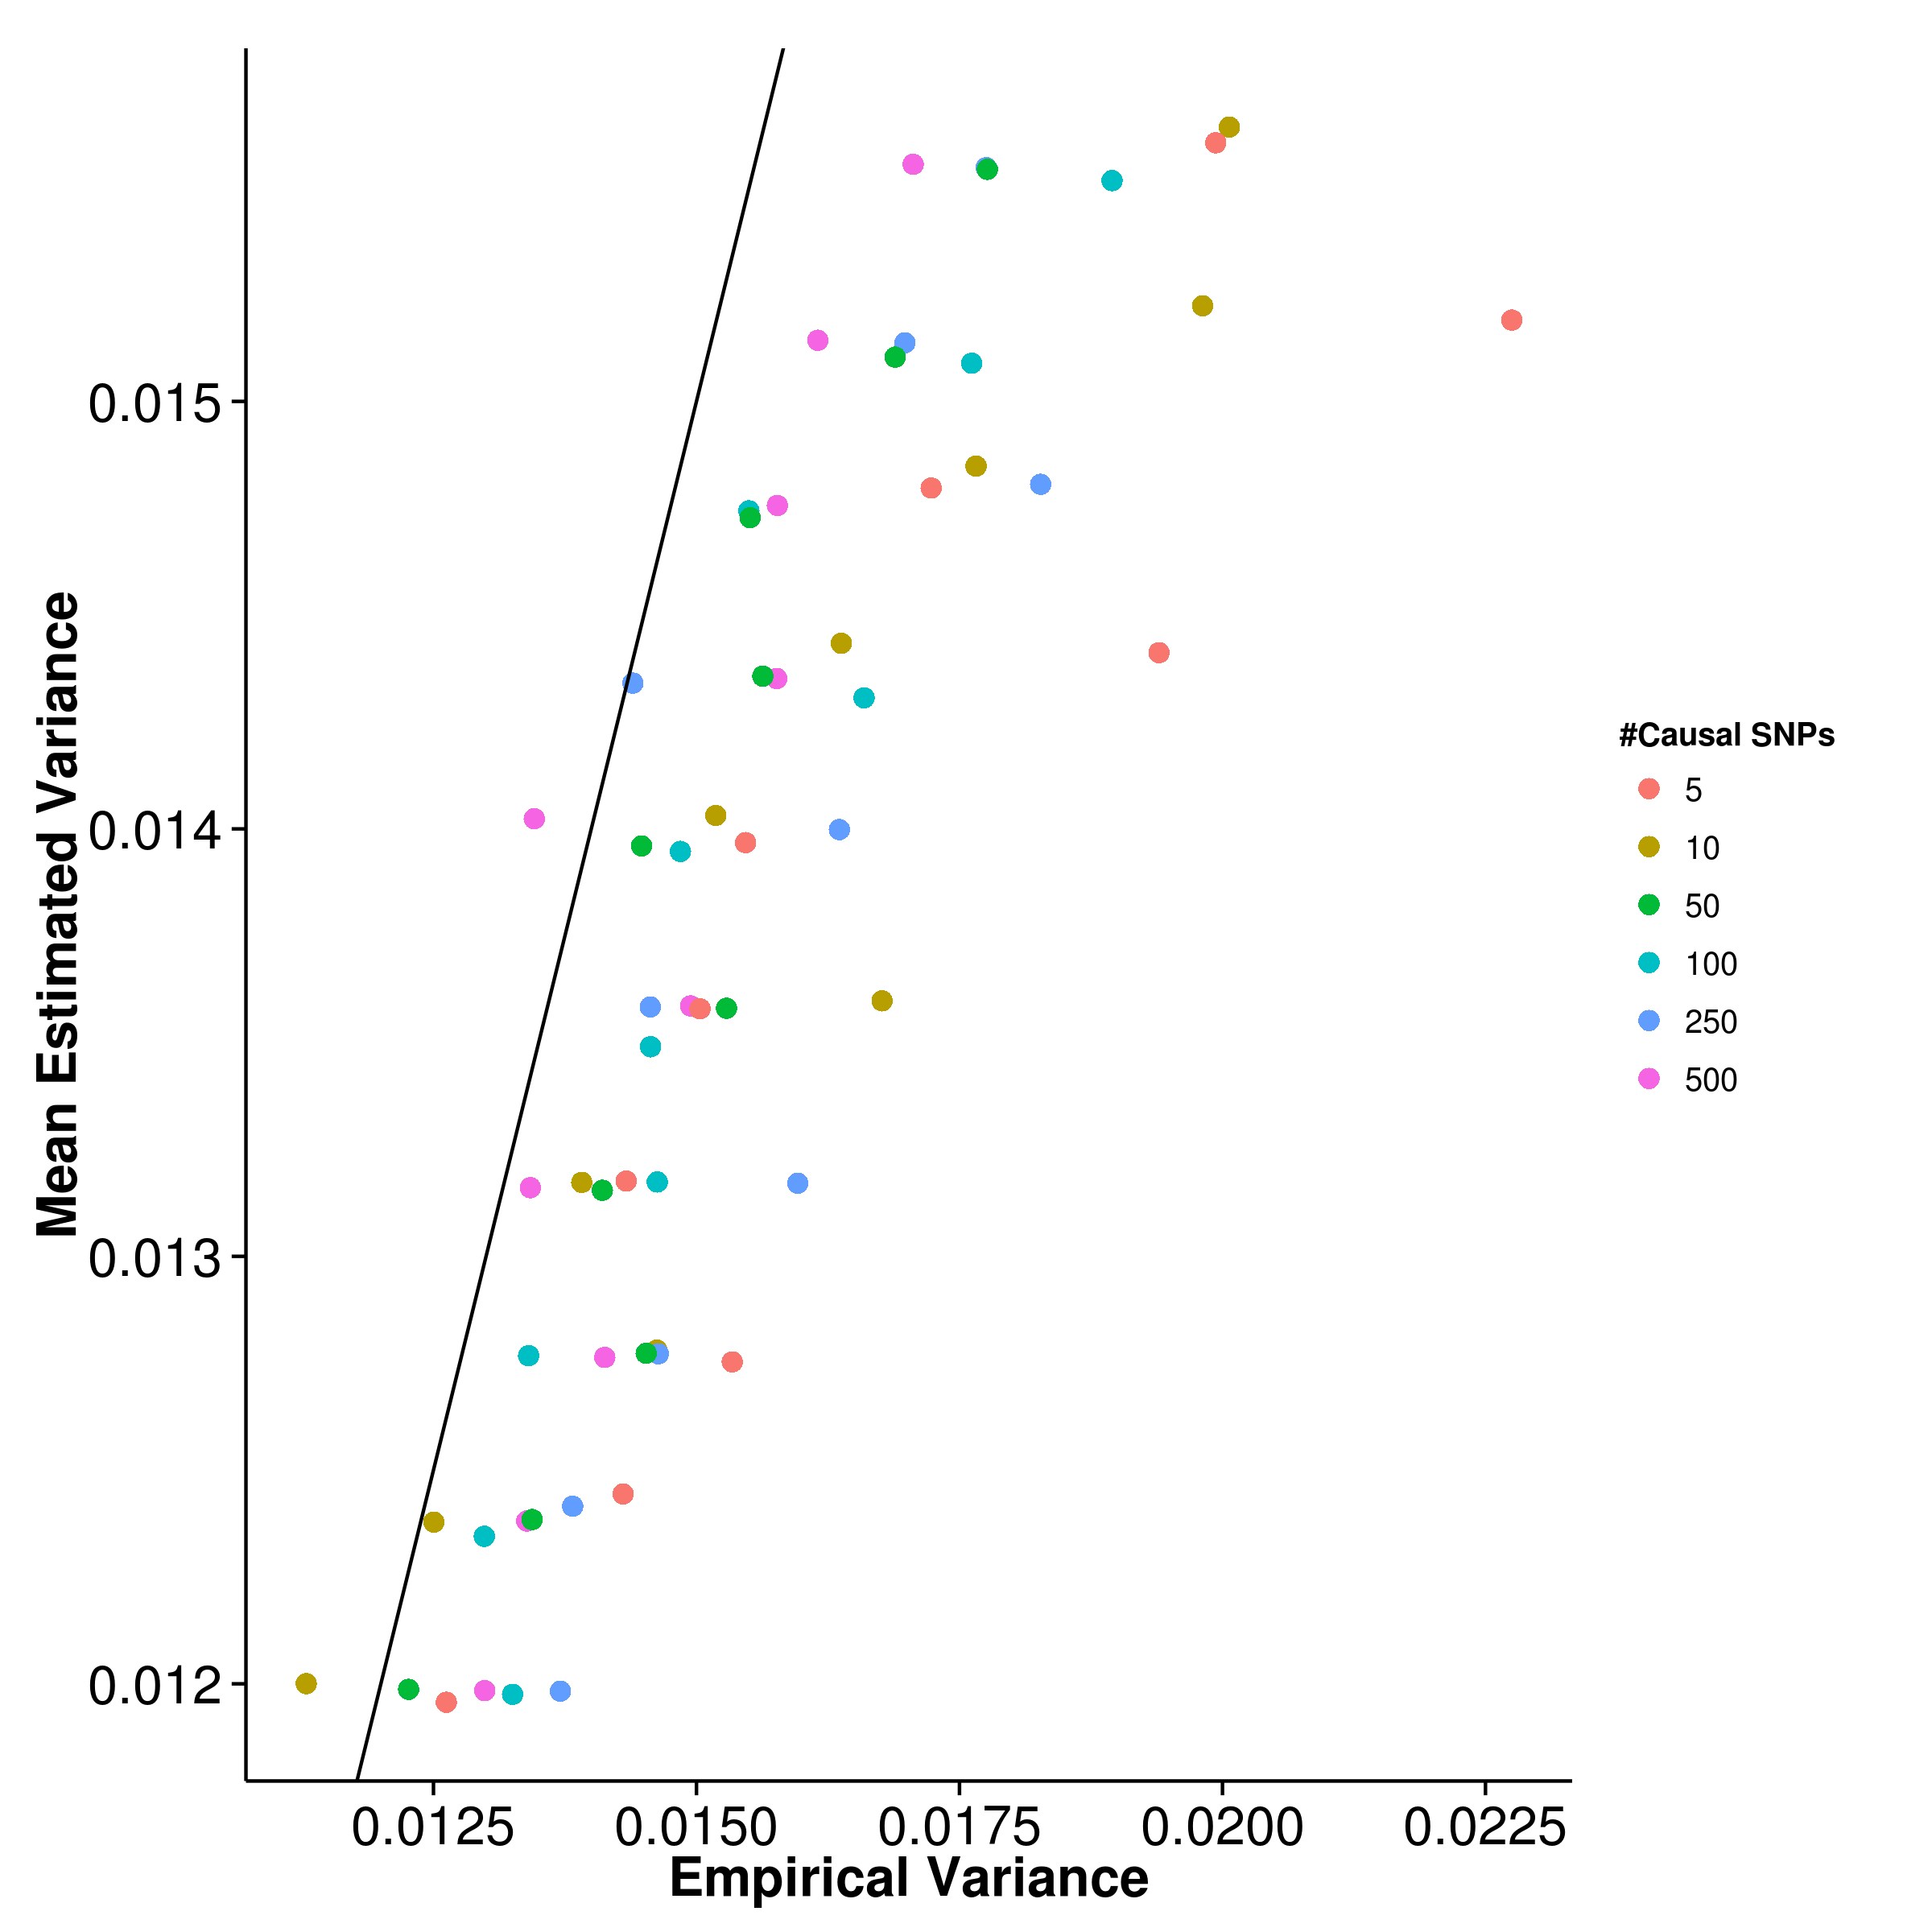
\includegraphics{figure/he_summary/equal/shrek_Qt_Equal_sdCom.png}}
				\label{fig:shrekQtEqualVarCom}
			}
			\subfloat[GCTA]{
				\scalebox{.4}{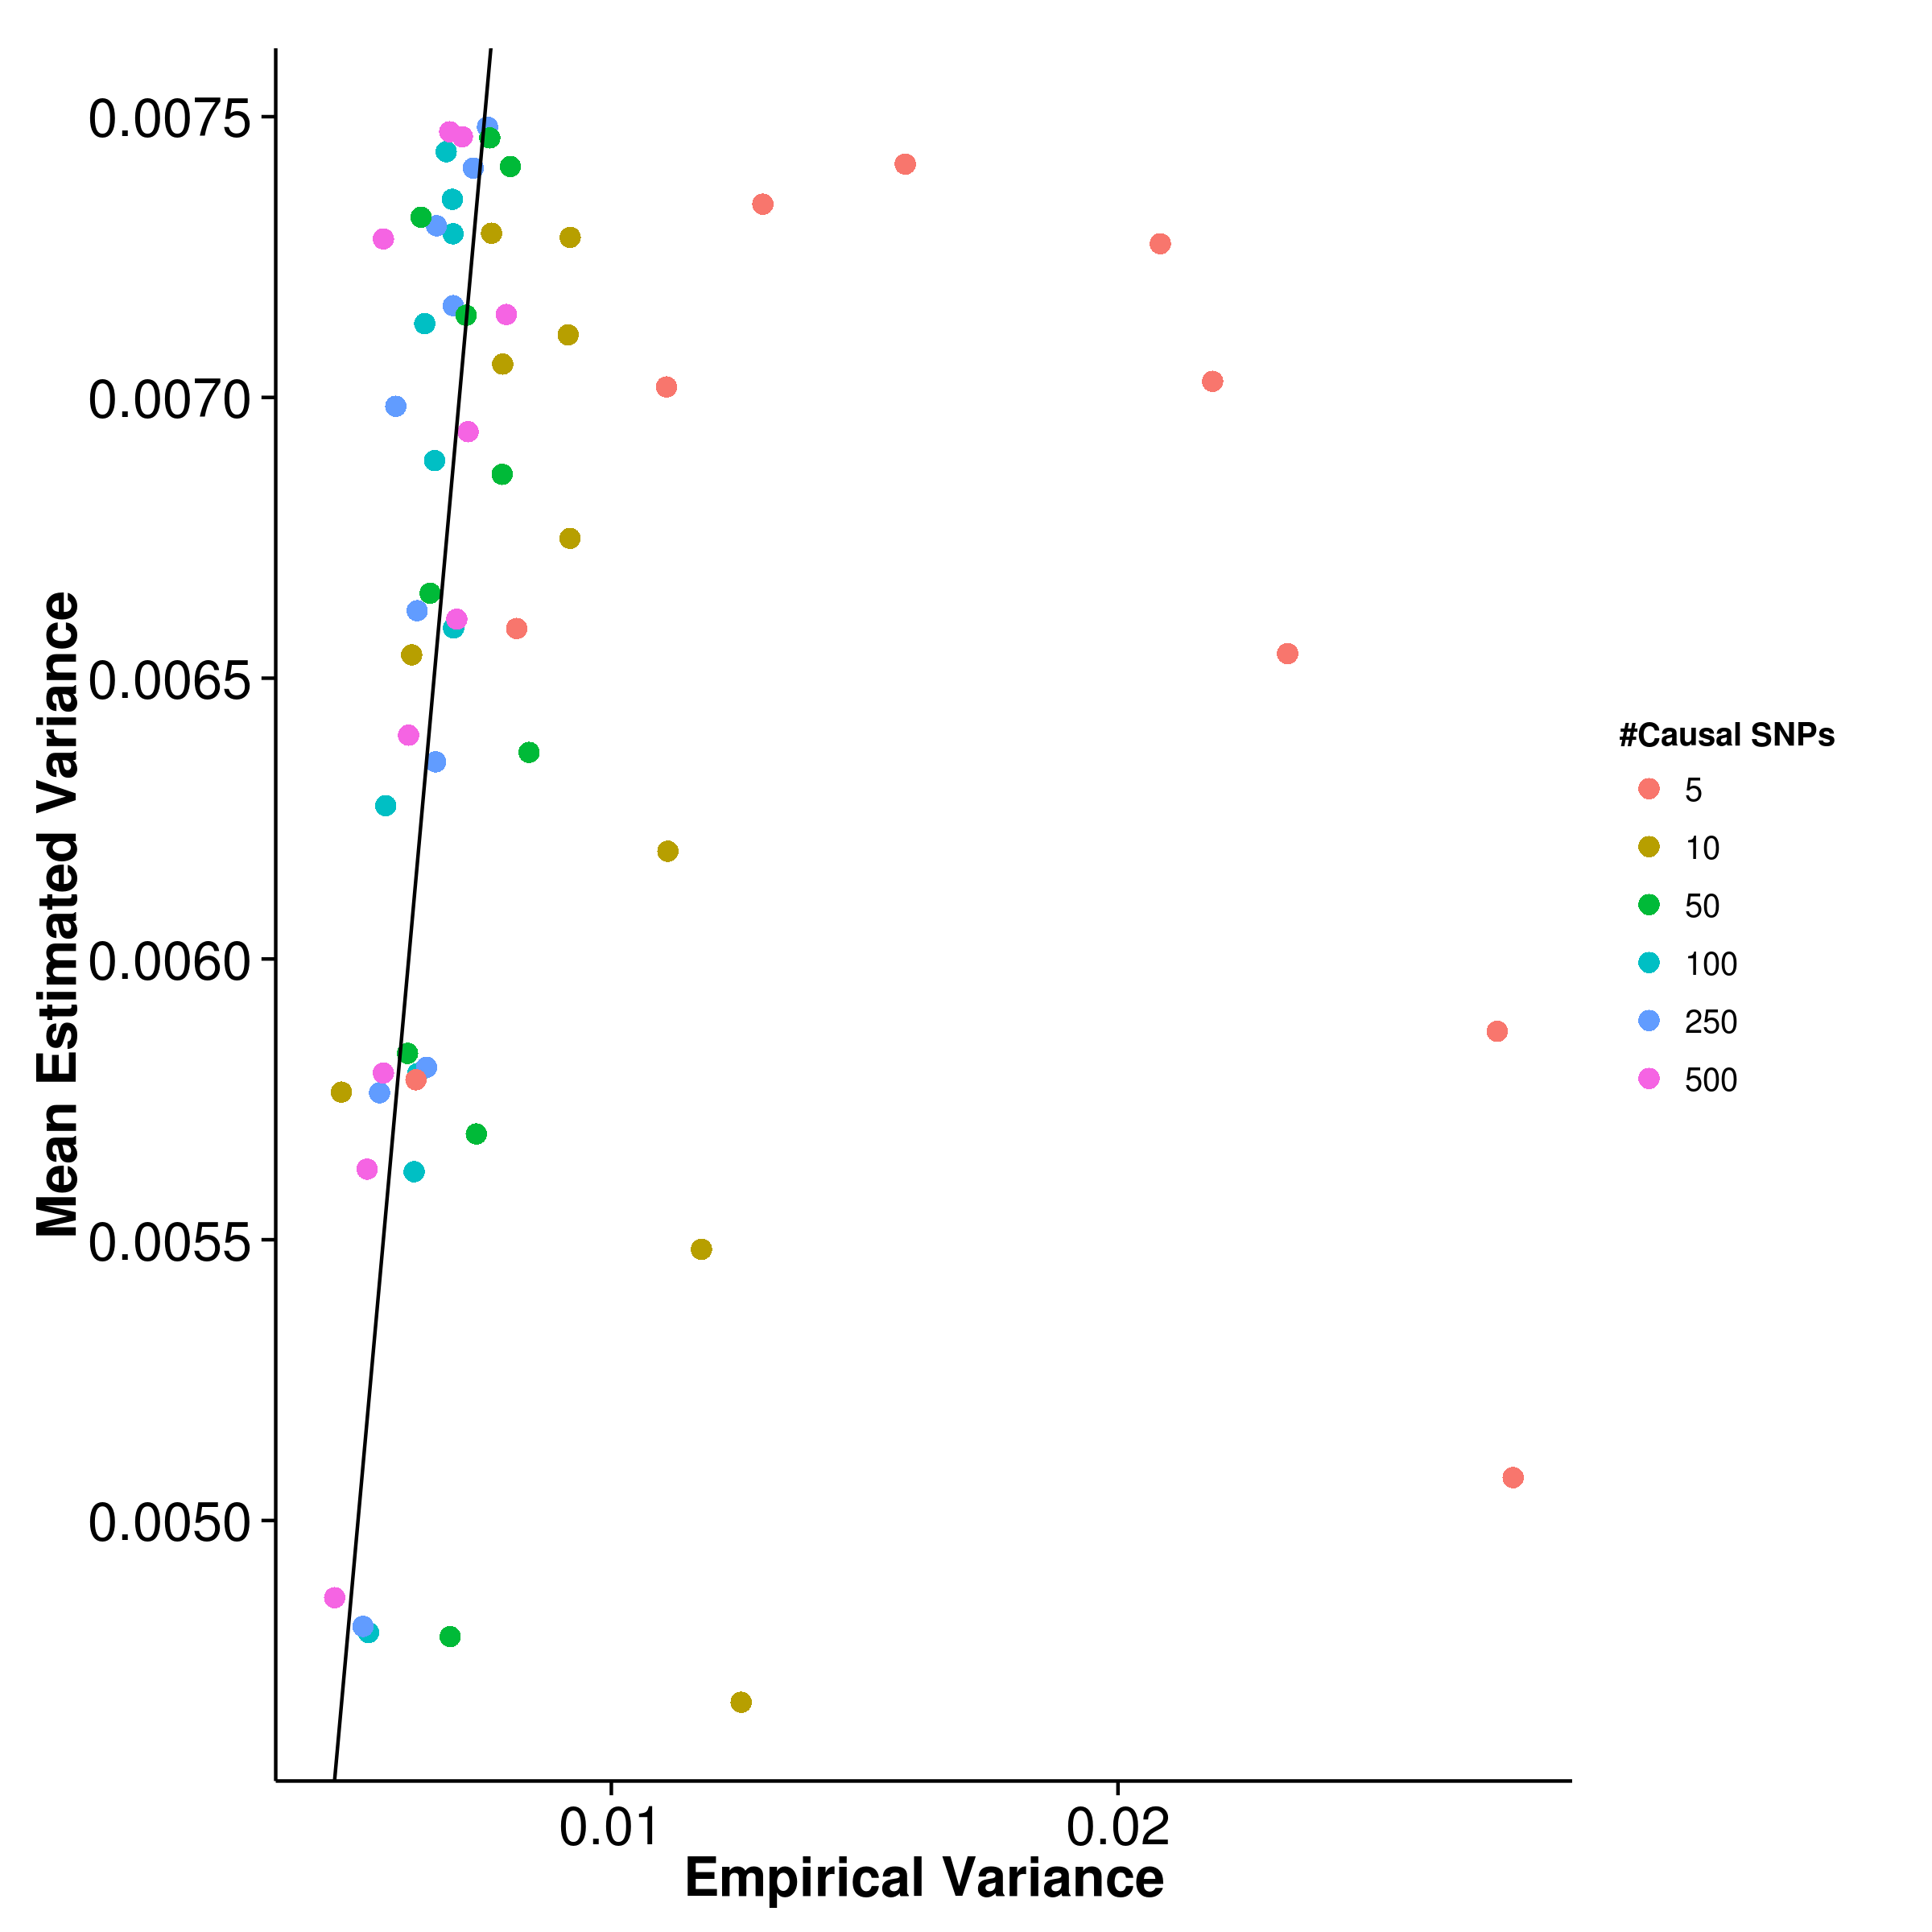
\includegraphics{figure/he_summary/equal/gcta_Qt_Equal_sdCom.png}}
				\label{fig:gctaQtEqualVarCom}
			}\\
			\subfloat[LDSC with fix intercept]{
				\scalebox{.4}{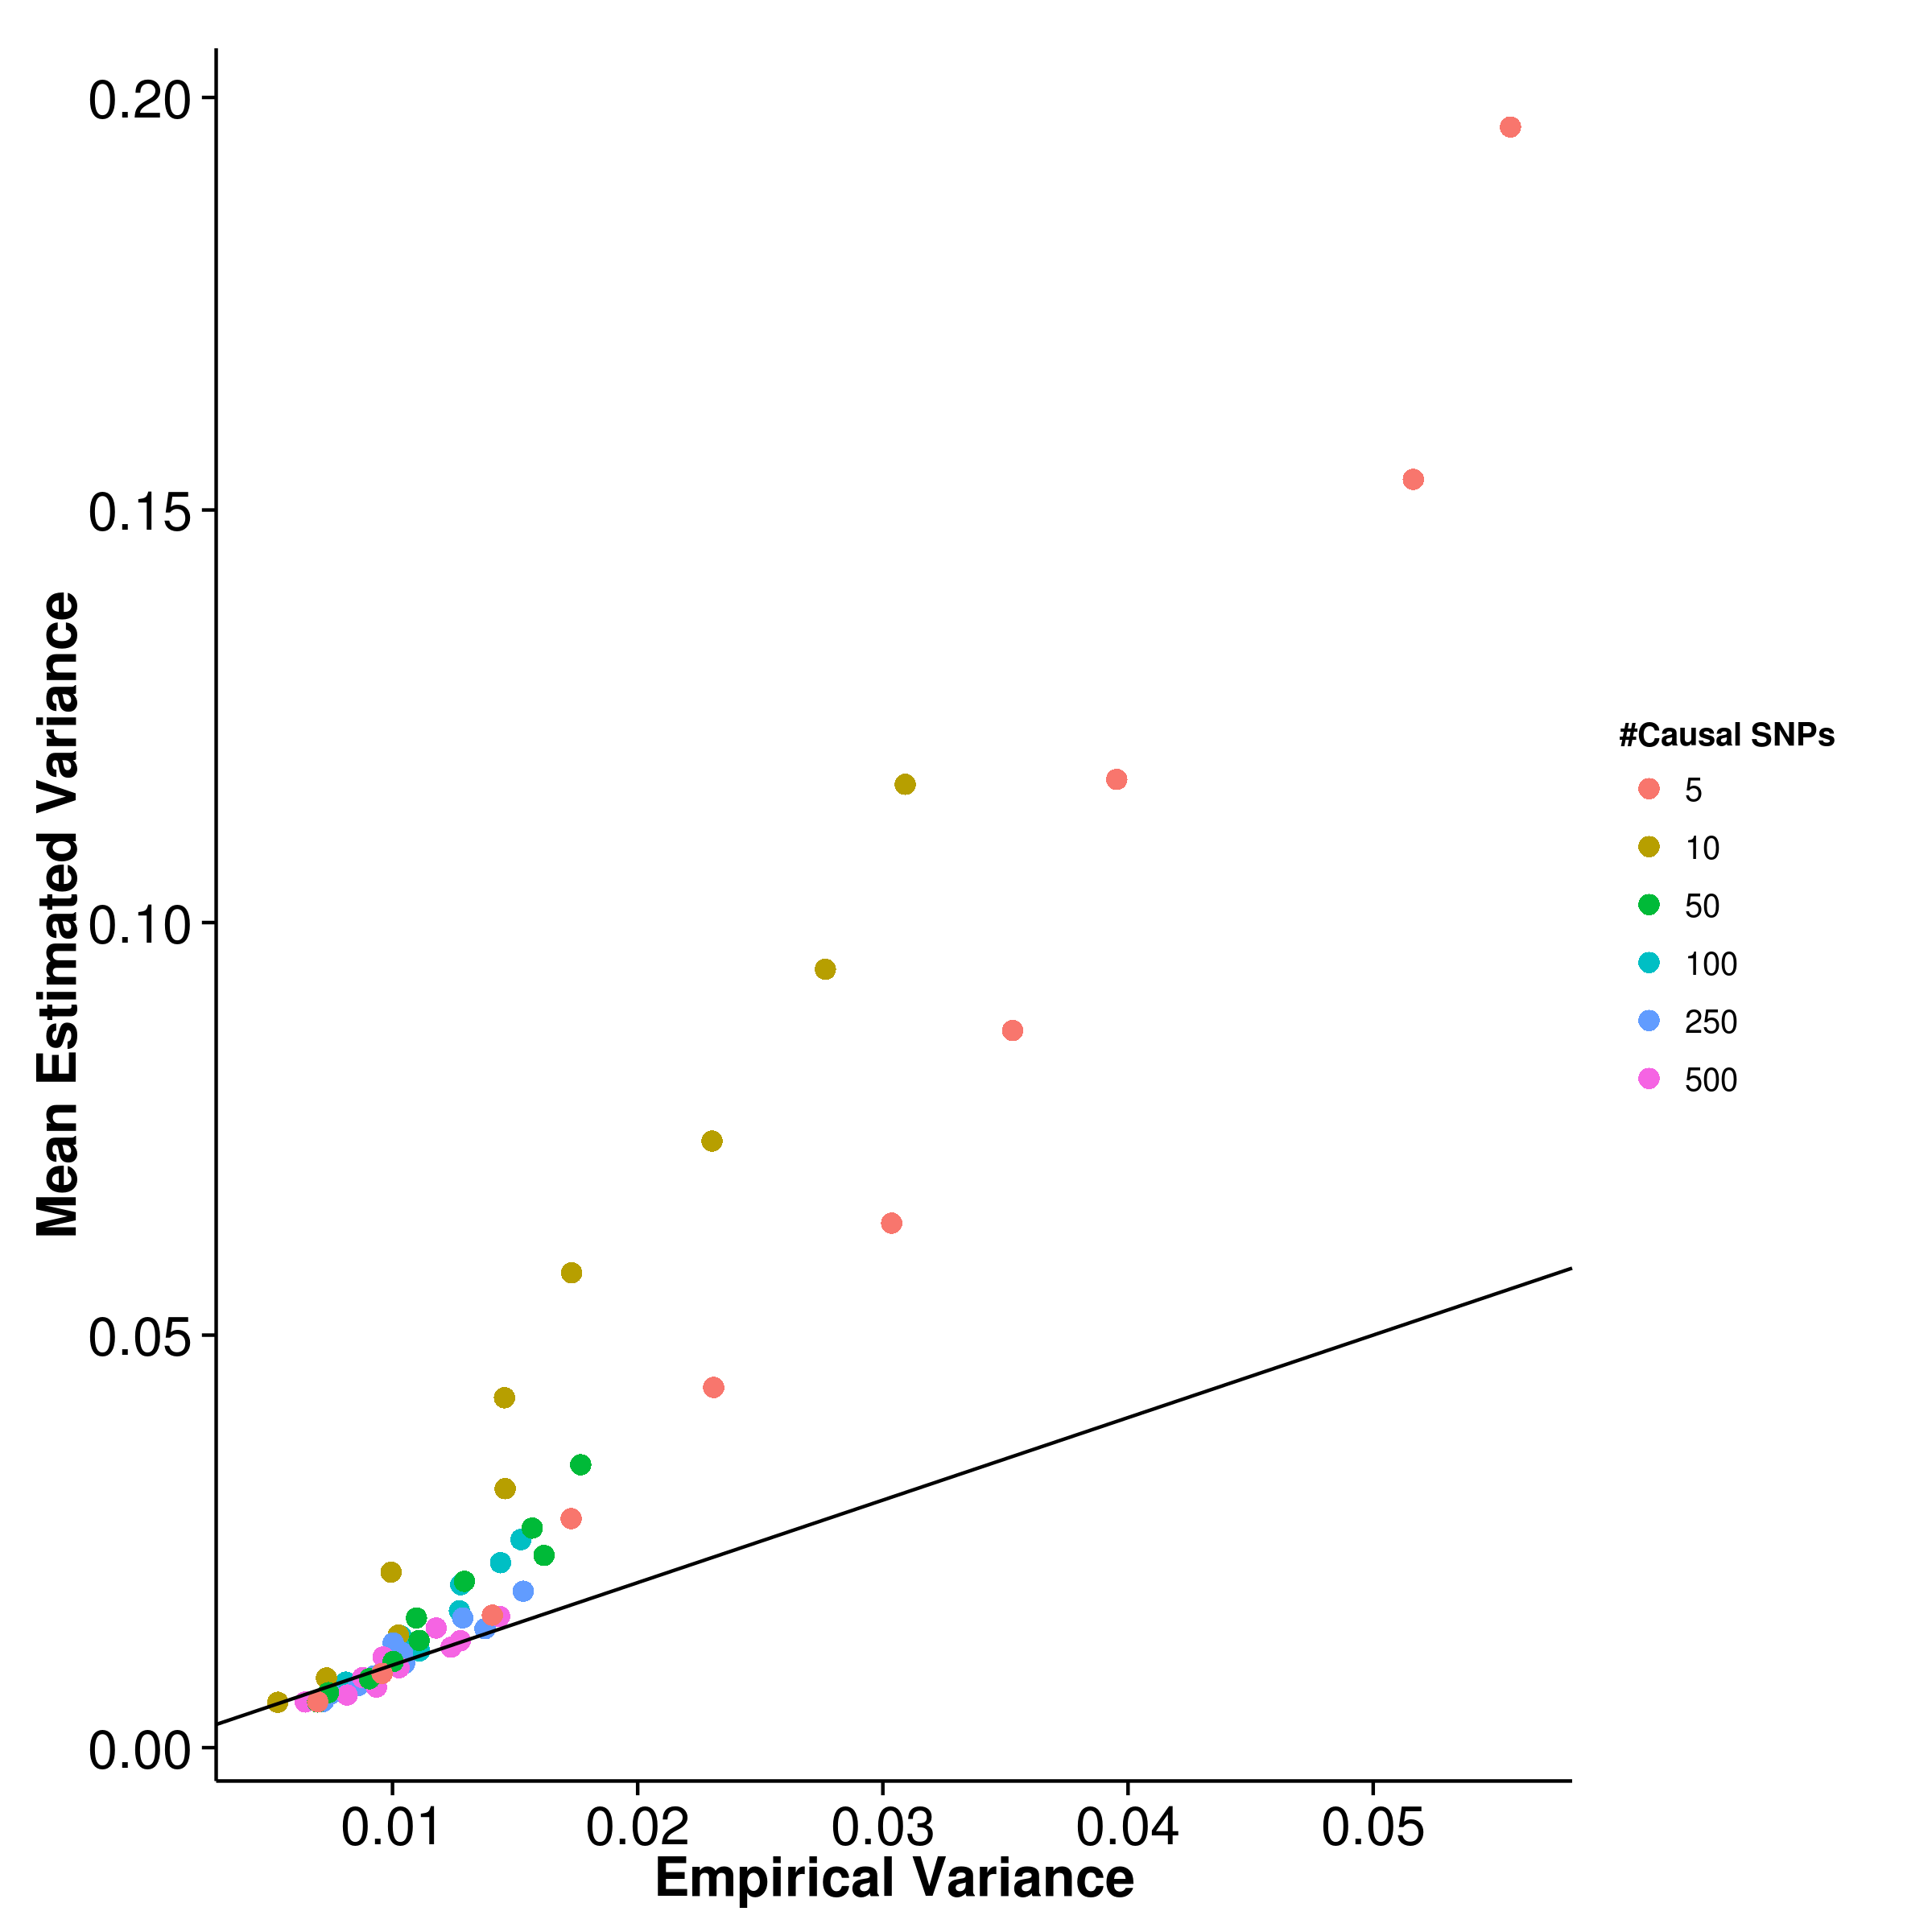
\includegraphics{figure/he_summary/equal/ldsc_Qt_Equal_sdCom.png}}
				\label{fig:ldscQtEqualVarCom}
			}
			\subfloat[LDSC with intercept estimation]{
				
				\scalebox{.4}{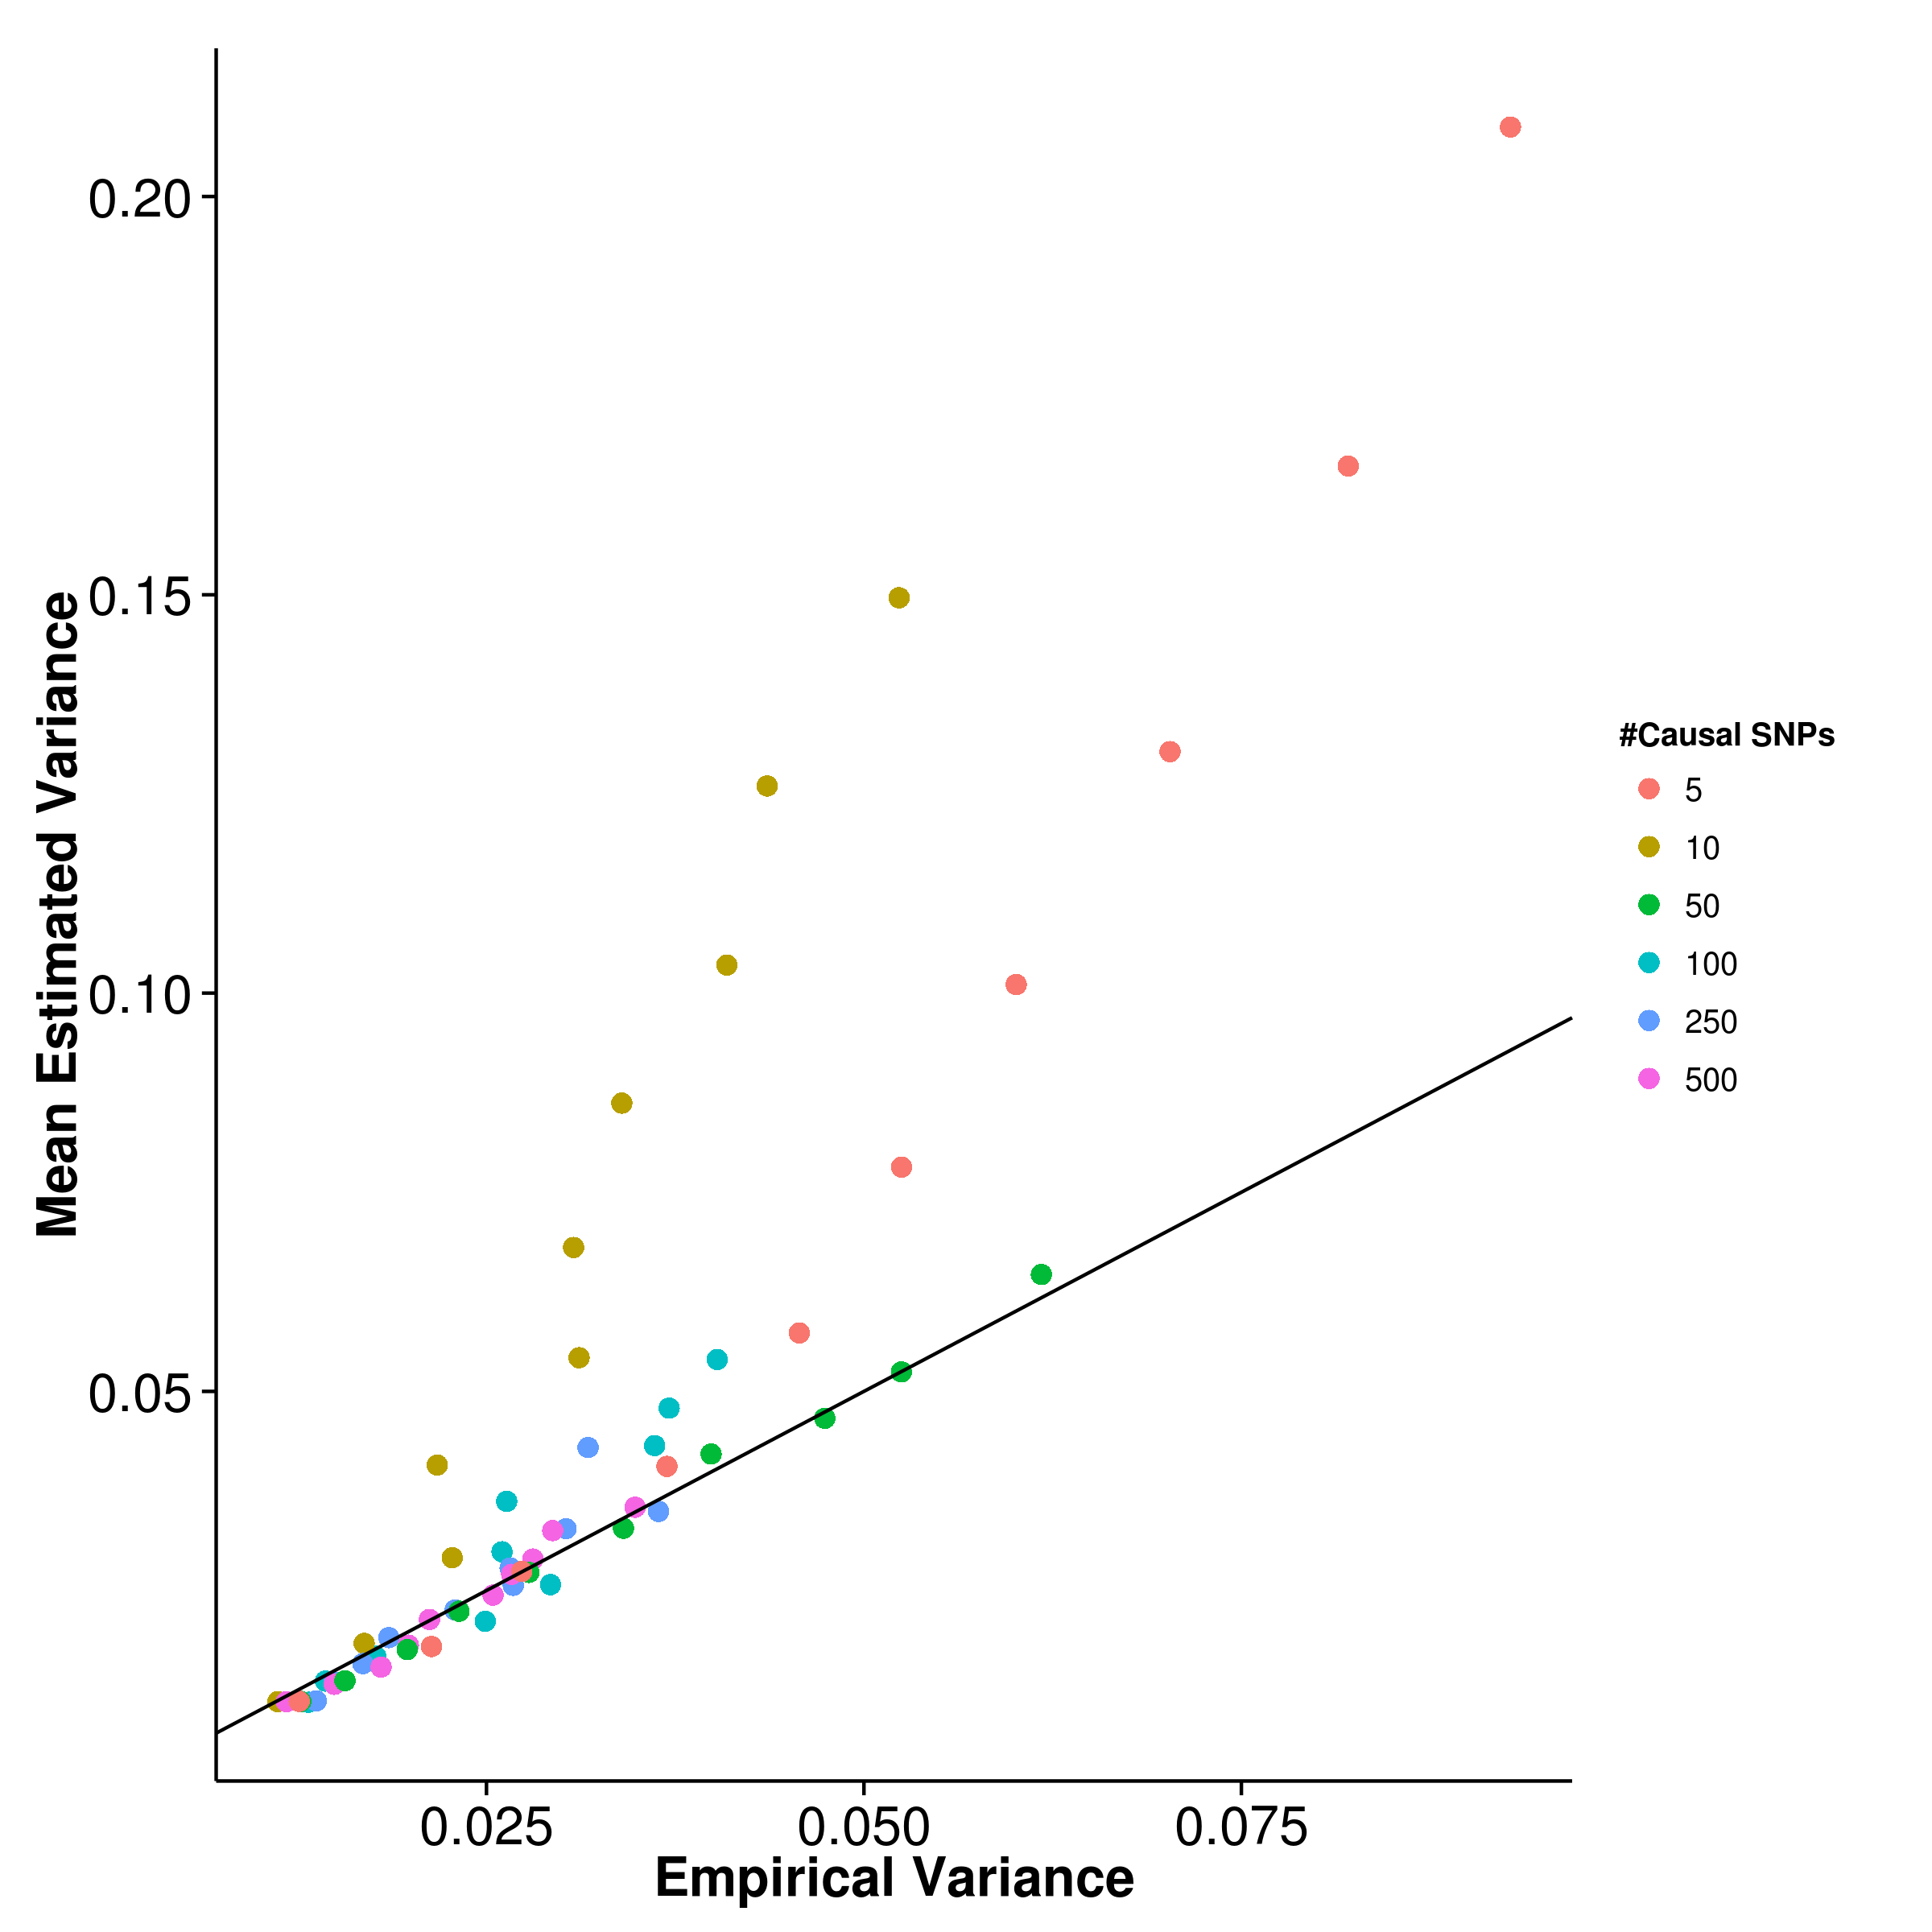
\includegraphics{figure/he_summary/equal/ldscIn_Qt_Equal_sdCom.png}}
				\label{fig:ldscInQtEqualVarCom}
			}
			\caption[Quantitative Trait with Equal Effect Size Simulation Result(Estimated Variance)]
			{Estimated variance of results from quantitative trait simulation with equal effect size simulation compared to the empirical variance.
				The estimated variances of all the tools were rather sensitive to the number of causal \glspl{SNP}, where \gls{ldsc} tends to over-estimate the variance as the number of causal \glspl{SNP} decreases and \gls{shrek} and \gls{gcta} tends to under-estimate the variance.} 
			\label{fig:QtEqualVarCom}
		\end{figure}